% Options for packages loaded elsewhere
% Options for packages loaded elsewhere
\PassOptionsToPackage{unicode}{hyperref}
\PassOptionsToPackage{hyphens}{url}
\PassOptionsToPackage{dvipsnames,svgnames,x11names}{xcolor}
%
\documentclass[
  russian,
  letterpaper,
  DIV=11,
  numbers=noendperiod]{scrartcl}
\usepackage{xcolor}
\usepackage{amsmath,amssymb}
\setcounter{secnumdepth}{5}
\usepackage{iftex}
\ifPDFTeX
  \usepackage[T1]{fontenc}
  \usepackage[utf8]{inputenc}
  \usepackage{textcomp} % provide euro and other symbols
\else % if luatex or xetex
  \usepackage{unicode-math} % this also loads fontspec
  \defaultfontfeatures{Scale=MatchLowercase}
  \defaultfontfeatures[\rmfamily]{Ligatures=TeX,Scale=1}
\fi
\usepackage{lmodern}
\ifPDFTeX\else
  % xetex/luatex font selection
\fi
% Use upquote if available, for straight quotes in verbatim environments
\IfFileExists{upquote.sty}{\usepackage{upquote}}{}
\IfFileExists{microtype.sty}{% use microtype if available
  \usepackage[]{microtype}
  \UseMicrotypeSet[protrusion]{basicmath} % disable protrusion for tt fonts
}{}
\makeatletter
\@ifundefined{KOMAClassName}{% if non-KOMA class
  \IfFileExists{parskip.sty}{%
    \usepackage{parskip}
  }{% else
    \setlength{\parindent}{0pt}
    \setlength{\parskip}{6pt plus 2pt minus 1pt}}
}{% if KOMA class
  \KOMAoptions{parskip=half}}
\makeatother
% Make \paragraph and \subparagraph free-standing
\makeatletter
\ifx\paragraph\undefined\else
  \let\oldparagraph\paragraph
  \renewcommand{\paragraph}{
    \@ifstar
      \xxxParagraphStar
      \xxxParagraphNoStar
  }
  \newcommand{\xxxParagraphStar}[1]{\oldparagraph*{#1}\mbox{}}
  \newcommand{\xxxParagraphNoStar}[1]{\oldparagraph{#1}\mbox{}}
\fi
\ifx\subparagraph\undefined\else
  \let\oldsubparagraph\subparagraph
  \renewcommand{\subparagraph}{
    \@ifstar
      \xxxSubParagraphStar
      \xxxSubParagraphNoStar
  }
  \newcommand{\xxxSubParagraphStar}[1]{\oldsubparagraph*{#1}\mbox{}}
  \newcommand{\xxxSubParagraphNoStar}[1]{\oldsubparagraph{#1}\mbox{}}
\fi
\makeatother

\usepackage{color}
\usepackage{fancyvrb}
\newcommand{\VerbBar}{|}
\newcommand{\VERB}{\Verb[commandchars=\\\{\}]}
\DefineVerbatimEnvironment{Highlighting}{Verbatim}{commandchars=\\\{\}}
% Add ',fontsize=\small' for more characters per line
\usepackage{framed}
\definecolor{shadecolor}{RGB}{241,243,245}
\newenvironment{Shaded}{\begin{snugshade}}{\end{snugshade}}
\newcommand{\AlertTok}[1]{\textcolor[rgb]{0.68,0.00,0.00}{#1}}
\newcommand{\AnnotationTok}[1]{\textcolor[rgb]{0.37,0.37,0.37}{#1}}
\newcommand{\AttributeTok}[1]{\textcolor[rgb]{0.40,0.45,0.13}{#1}}
\newcommand{\BaseNTok}[1]{\textcolor[rgb]{0.68,0.00,0.00}{#1}}
\newcommand{\BuiltInTok}[1]{\textcolor[rgb]{0.00,0.23,0.31}{#1}}
\newcommand{\CharTok}[1]{\textcolor[rgb]{0.13,0.47,0.30}{#1}}
\newcommand{\CommentTok}[1]{\textcolor[rgb]{0.37,0.37,0.37}{#1}}
\newcommand{\CommentVarTok}[1]{\textcolor[rgb]{0.37,0.37,0.37}{\textit{#1}}}
\newcommand{\ConstantTok}[1]{\textcolor[rgb]{0.56,0.35,0.01}{#1}}
\newcommand{\ControlFlowTok}[1]{\textcolor[rgb]{0.00,0.23,0.31}{\textbf{#1}}}
\newcommand{\DataTypeTok}[1]{\textcolor[rgb]{0.68,0.00,0.00}{#1}}
\newcommand{\DecValTok}[1]{\textcolor[rgb]{0.68,0.00,0.00}{#1}}
\newcommand{\DocumentationTok}[1]{\textcolor[rgb]{0.37,0.37,0.37}{\textit{#1}}}
\newcommand{\ErrorTok}[1]{\textcolor[rgb]{0.68,0.00,0.00}{#1}}
\newcommand{\ExtensionTok}[1]{\textcolor[rgb]{0.00,0.23,0.31}{#1}}
\newcommand{\FloatTok}[1]{\textcolor[rgb]{0.68,0.00,0.00}{#1}}
\newcommand{\FunctionTok}[1]{\textcolor[rgb]{0.28,0.35,0.67}{#1}}
\newcommand{\ImportTok}[1]{\textcolor[rgb]{0.00,0.46,0.62}{#1}}
\newcommand{\InformationTok}[1]{\textcolor[rgb]{0.37,0.37,0.37}{#1}}
\newcommand{\KeywordTok}[1]{\textcolor[rgb]{0.00,0.23,0.31}{\textbf{#1}}}
\newcommand{\NormalTok}[1]{\textcolor[rgb]{0.00,0.23,0.31}{#1}}
\newcommand{\OperatorTok}[1]{\textcolor[rgb]{0.37,0.37,0.37}{#1}}
\newcommand{\OtherTok}[1]{\textcolor[rgb]{0.00,0.23,0.31}{#1}}
\newcommand{\PreprocessorTok}[1]{\textcolor[rgb]{0.68,0.00,0.00}{#1}}
\newcommand{\RegionMarkerTok}[1]{\textcolor[rgb]{0.00,0.23,0.31}{#1}}
\newcommand{\SpecialCharTok}[1]{\textcolor[rgb]{0.37,0.37,0.37}{#1}}
\newcommand{\SpecialStringTok}[1]{\textcolor[rgb]{0.13,0.47,0.30}{#1}}
\newcommand{\StringTok}[1]{\textcolor[rgb]{0.13,0.47,0.30}{#1}}
\newcommand{\VariableTok}[1]{\textcolor[rgb]{0.07,0.07,0.07}{#1}}
\newcommand{\VerbatimStringTok}[1]{\textcolor[rgb]{0.13,0.47,0.30}{#1}}
\newcommand{\WarningTok}[1]{\textcolor[rgb]{0.37,0.37,0.37}{\textit{#1}}}

\usepackage{longtable,booktabs,array}
\usepackage{calc} % for calculating minipage widths
% Correct order of tables after \paragraph or \subparagraph
\usepackage{etoolbox}
\makeatletter
\patchcmd\longtable{\par}{\if@noskipsec\mbox{}\fi\par}{}{}
\makeatother
% Allow footnotes in longtable head/foot
\IfFileExists{footnotehyper.sty}{\usepackage{footnotehyper}}{\usepackage{footnote}}
\makesavenoteenv{longtable}
\usepackage{graphicx}
\makeatletter
\newsavebox\pandoc@box
\newcommand*\pandocbounded[1]{% scales image to fit in text height/width
  \sbox\pandoc@box{#1}%
  \Gscale@div\@tempa{\textheight}{\dimexpr\ht\pandoc@box+\dp\pandoc@box\relax}%
  \Gscale@div\@tempb{\linewidth}{\wd\pandoc@box}%
  \ifdim\@tempb\p@<\@tempa\p@\let\@tempa\@tempb\fi% select the smaller of both
  \ifdim\@tempa\p@<\p@\scalebox{\@tempa}{\usebox\pandoc@box}%
  \else\usebox{\pandoc@box}%
  \fi%
}
% Set default figure placement to htbp
\def\fps@figure{htbp}
\makeatother



\ifLuaTeX
\usepackage[bidi=basic,provide=*]{babel}
\else
\usepackage[bidi=default,provide=*]{babel}
\fi
% get rid of language-specific shorthands (see #6817):
\let\LanguageShortHands\languageshorthands
\def\languageshorthands#1{}


\setlength{\emergencystretch}{3em} % prevent overfull lines

\providecommand{\tightlist}{%
  \setlength{\itemsep}{0pt}\setlength{\parskip}{0pt}}



 


\usepackage{fontspec}

\setsansfont{Palatino Linotype}[
    Path=../files/palatino/,
    Extension = .ttf,
    UprightFont=palatino-Roman,
    BoldFont=palatino-Bold,
    ItalicFont=palatino-Italic,
    BoldItalicFont=palatino-BoldItalic
]
\setmainfont{Palatino Linotype}[
    Path=../files/palatino/,
    Extension = .ttf,
    UprightFont=palatino-Roman,
    BoldFont=palatino-Bold,
    ItalicFont=palatino-Italic,
    BoldItalicFont=palatino-BoldItalic
]

\usepackage[textwidth=0.86\paperwidth, textheight=0.86\paperheight]{geometry}
\usepackage{fancyhdr}
\usepackage{hyperref}
\usepackage{fontawesome5}
\usepackage{graphicx}
\usepackage{amssymb}
\usepackage{amsmath}
\graphicspath{{../files/}}

\newcommand{\R}{\mathbb{R}}

% \pagenumbering{gobble}
\pagestyle{fancy}
\fancyhead{} % clear all header fields
\fancyhead[R]{\href{https://cu25.fmin.xyz}{\faGem[regular]} \hspace{0.04cm} \href{https://github.com/MerkulovDaniil/cu25}{\faGithub} \hspace{0.07cm} \href{https://t.me/fminxyz}{\faTelegram}}
\fancyhead[L]{\href{https://fmin.xyz}{
\includegraphics[height=0.35cm]{logo.pdf}} ~ 
\includegraphics[height=0.35cm]{logo_cu.pdf} \hspace{2pt} \textbf{Оптимизация для всех! ЦУ. 2025}}
\KOMAoption{captions}{tableheading}
\makeatletter
\@ifpackageloaded{tcolorbox}{}{\usepackage[skins,breakable]{tcolorbox}}
\@ifpackageloaded{fontawesome5}{}{\usepackage{fontawesome5}}
\definecolor{quarto-callout-color}{HTML}{909090}
\definecolor{quarto-callout-note-color}{HTML}{0758E5}
\definecolor{quarto-callout-important-color}{HTML}{CC1914}
\definecolor{quarto-callout-warning-color}{HTML}{EB9113}
\definecolor{quarto-callout-tip-color}{HTML}{00A047}
\definecolor{quarto-callout-caution-color}{HTML}{FC5300}
\definecolor{quarto-callout-color-frame}{HTML}{acacac}
\definecolor{quarto-callout-note-color-frame}{HTML}{4582ec}
\definecolor{quarto-callout-important-color-frame}{HTML}{d9534f}
\definecolor{quarto-callout-warning-color-frame}{HTML}{f0ad4e}
\definecolor{quarto-callout-tip-color-frame}{HTML}{02b875}
\definecolor{quarto-callout-caution-color-frame}{HTML}{fd7e14}
\makeatother
\makeatletter
\@ifpackageloaded{caption}{}{\usepackage{caption}}
\AtBeginDocument{%
\ifdefined\contentsname
  \renewcommand*\contentsname{Содержание}
\else
  \newcommand\contentsname{Содержание}
\fi
\ifdefined\listfigurename
  \renewcommand*\listfigurename{Список Иллюстраций}
\else
  \newcommand\listfigurename{Список Иллюстраций}
\fi
\ifdefined\listtablename
  \renewcommand*\listtablename{Список Таблиц}
\else
  \newcommand\listtablename{Список Таблиц}
\fi
\ifdefined\figurename
  \renewcommand*\figurename{Рисунок}
\else
  \newcommand\figurename{Рисунок}
\fi
\ifdefined\tablename
  \renewcommand*\tablename{Таблица}
\else
  \newcommand\tablename{Таблица}
\fi
}
\@ifpackageloaded{float}{}{\usepackage{float}}
\floatstyle{ruled}
\@ifundefined{c@chapter}{\newfloat{codelisting}{h}{lop}}{\newfloat{codelisting}{h}{lop}[chapter]}
\floatname{codelisting}{Список}
\newcommand*\listoflistings{\listof{codelisting}{Список Каталогов}}
\makeatother
\makeatletter
\makeatother
\makeatletter
\@ifpackageloaded{caption}{}{\usepackage{caption}}
\@ifpackageloaded{subcaption}{}{\usepackage{subcaption}}
\makeatother
\usepackage{bookmark}
\IfFileExists{xurl.sty}{\usepackage{xurl}}{} % add URL line breaks if available
\urlstyle{same}
\hypersetup{
  pdftitle={Нижние оценки для градиентного спуска. Ускоренный градиентный спуск. Момент. Ускорение Нестерова},
  pdfauthor={Даня Меркулов},
  pdflang={ru},
  colorlinks=true,
  linkcolor={blue},
  filecolor={Maroon},
  citecolor={Blue},
  urlcolor={Blue},
  pdfcreator={LaTeX via pandoc}}


\title{Нижние оценки для градиентного спуска. Ускоренный градиентный
спуск. Момент. Ускорение Нестерова}
\author{Даня Меркулов}
\date{}
\begin{document}
\maketitle


\section{Сходимость градиентного
спуска}\label{ux441ux445ux43eux434ux438ux43cux43eux441ux442ux44c-ux433ux440ux430ux434ux438ux435ux43dux442ux43dux43eux433ux43e-ux441ux43fux443ux441ux43aux430}

\[
\text{Градиентный спуск:} \qquad \qquad \min_{x \in \mathbb{R}^n} f(x) \qquad \qquad x_{k+1} = x_k - \alpha_k \nabla f(x_k)
\]

\begin{longtable}[]{@{}
  >{\centering\arraybackslash}p{(\linewidth - 6\tabcolsep) * \real{0.2286}}
  >{\centering\arraybackslash}p{(\linewidth - 6\tabcolsep) * \real{0.2571}}
  >{\centering\arraybackslash}p{(\linewidth - 6\tabcolsep) * \real{0.2286}}
  >{\centering\arraybackslash}p{(\linewidth - 6\tabcolsep) * \real{0.2857}}@{}}
\toprule\noalign{}
\begin{minipage}[b]{\linewidth}\centering
выпуклая (негладкая)
\end{minipage} & \begin{minipage}[b]{\linewidth}\centering
гладкая (невыпуклая)
\end{minipage} & \begin{minipage}[b]{\linewidth}\centering
гладкая \& выпуклая
\end{minipage} & \begin{minipage}[b]{\linewidth}\centering
гладкая \& сильно выпуклая
\end{minipage} \\
\midrule\noalign{}
\endhead
\bottomrule\noalign{}
\endlastfoot
\(f(x_k) - f^* =  \mathcal{O} \left( \tfrac{1}{\sqrt{k}} \right)\) &
\(\min\limits_{0 \leq i \leq k}\|\nabla f(x_i)\| = \mathcal{O} \left( \tfrac{1}{\sqrt{k}} \right)\)
& \(f(x_k) - f^* =  \mathcal{O} \left( \tfrac{1}{k} \right)\) &
\(\|x_k - x^*\|^2 = \mathcal{O} \left( \left(1 - \tfrac{\mu}{L}\right)^k \right)\) \\
\(k_\varepsilon =  \mathcal{O} \left( \tfrac{1}{\varepsilon^2} \right)\)
&
\(k_\varepsilon = \mathcal{O} \left( \tfrac{1}{\varepsilon^2} \right)\)
&
\(k_\varepsilon =  \mathcal{O}  \left( \tfrac{1}{\varepsilon} \right)\)
&
\(k_\varepsilon  = \mathcal{O} \left( \varkappa \log \tfrac{1}{\varepsilon}\right)\) \\
\end{longtable}

Для гладкой сильно выпуклой функции мы имеем: \[
f(x_{k})-f^* \leq \left(1- \dfrac{\mu}{L}\right)^k (f(x_0)-f^*).
\]

Обратите внимание, что для любого \(x\), поскольку \(e^{-x}\) выпуклая и
\(1-x\) является её касательной в точке \(x=0\), мы имеем: \[
1 - x \leq e^{-x}
\]

Наконец: \[
\begin{aligned}
\varepsilon &= f(x_{k_\varepsilon})-f^* \leq  \left(1- \dfrac{\mu}{L}\right)^{k_\varepsilon} (f(x_0)-f^*) \\
&\leq \exp\left(- k_\varepsilon\dfrac{\mu}{L}\right) (f(x_0)-f^*) \\
k_\varepsilon &\geq \varkappa \log \dfrac{f(x_0)-f^*}{\varepsilon} = \mathcal{O} \left( \varkappa \log \dfrac{1}{\varepsilon}\right)
\end{aligned}
\]

\textbf{Вопрос: }Можно ли добиться лучшей скорости сходимости, используя
только информацию первого порядка? \textbf{Да, можно.}

\section{Нижние
оценки}\label{ux43dux438ux436ux43dux438ux435-ux43eux446ux435ux43dux43aux438}

Для нижних оценок пишут \(\Omega \left( \cdot \right)\) вместо
\(\mathcal{O} \left( \cdot \right)\).

\begin{longtable}[]{@{}
  >{\centering\arraybackslash}p{(\linewidth - 6\tabcolsep) * \real{0.2286}}
  >{\centering\arraybackslash}p{(\linewidth - 6\tabcolsep) * \real{0.2571}}
  >{\centering\arraybackslash}p{(\linewidth - 6\tabcolsep) * \real{0.2286}}
  >{\centering\arraybackslash}p{(\linewidth - 6\tabcolsep) * \real{0.2857}}@{}}
\toprule\noalign{}
\begin{minipage}[b]{\linewidth}\centering
выпуклая (негладкая)
\end{minipage} & \begin{minipage}[b]{\linewidth}\centering
гладкая (невыпуклая)\footnote{\href{https://arxiv.org/pdf/1710.11606.pdf}{Carmon,
  Duchi, Hinder, Sidford, 2017}}
\end{minipage} & \begin{minipage}[b]{\linewidth}\centering
гладкая \& выпуклая\footnote{\href{https://fmin.xyz/assets/files/nemyud1979.pdf}{Nemirovski,
  Yudin, 1979}}
\end{minipage} & \begin{minipage}[b]{\linewidth}\centering
гладкая \& сильно выпуклая
\end{minipage} \\
\midrule\noalign{}
\endhead
\bottomrule\noalign{}
\endlastfoot
\(f(x_k) - f^* =  \Omega \left( \tfrac{1}{\sqrt{k}} \right)\) &
\(\min\limits_{0 \leq i \leq k}\|\nabla f(x_i)\| = \Omega \left( \tfrac{1}{\sqrt{k}} \right)\)
& \(f(x_k)-f^*=\Omega\!\left(\tfrac{1}{k^2}\right)\) &
\(f(x_k)-f^*=\Omega\!\left(\left(\tfrac{\sqrt{\varkappa}-1}{\sqrt{\varkappa}+1}\right)^{\!2k}\right)\) \\
\(k_\varepsilon =  \Omega \left( \tfrac{1}{\varepsilon^2} \right)\) &
\(k_\varepsilon=\Omega\!\left(\tfrac{1}{\varepsilon^2}\right)\) &
\(k_\varepsilon=\Omega\!\left(\tfrac{1}{\sqrt{\varepsilon}}\right)\) &
\(k_\varepsilon=\Omega\!\big(\sqrt{\varkappa}\,\log\tfrac{1}{\varepsilon}\big)\) \\
\end{longtable}

\subsection{Чёрный
ящик}\label{ux447ux451ux440ux43dux44bux439-ux44fux449ux438ux43a}

Итерация градиентного спуска: \[
\begin{aligned}
x_{k+1} &= x_k - \alpha_k \nabla f(x_k)  \\ 
&= x_{k-1} - \alpha_{k-1} \nabla f(x_{k-1}) - \alpha_k \nabla f(x_k) \\ 
& \;\;\vdots  \\ 
&= x_0 - \sum\limits_{i=0}^k \alpha_{k-i} \nabla f(x_{k-i})
\end{aligned}
\]

Рассмотрим семейство методов первого порядка, где
\begin{equation}\phantomsection\label{eq-fom}{
\begin{aligned}
x_{k+1} &\in x_0 + \text{Lin} \left\{\nabla f(x_0), \nabla f(x_1), \ldots, \nabla f(x_k)\right\} \; & f \text{ — гладкая} \\
x_{k+1} &\in x_0 + \text{Lin} \left\{g_{0}, g_{1}, \ldots, g_{k}\right\} \text{, где }
g_{i} \in \partial f(x_{i}) \; & f \text{ — негладкая}
\end{aligned}
}\end{equation}

Чтобы построить нижнюю оценку, нам нужно найти функцию \(f\) из
соответствующего класса, такую, что любой метод из семейства
(\ref{eq-fom}) будет работать не быстрее этой нижней оценки.

\subsection{Гладкий
случай}\label{ux433ux43bux430ux434ux43aux438ux439-ux441ux43bux443ux447ux430ux439}

\begin{tcolorbox}[enhanced jigsaw, rightrule=.15mm, coltitle=black, title=\textcolor{quarto-callout-color}{\faInfo}\hspace{0.5em}{Theorem}, colbacktitle=quarto-callout-color!10!white, opacityback=0, colframe=quarto-callout-color-frame, bottomtitle=1mm, toptitle=1mm, titlerule=0mm, arc=.35mm, leftrule=.75mm, breakable, toprule=.15mm, bottomrule=.15mm, opacitybacktitle=0.6, left=2mm, colback=white]

Существует \(L\)-гладкая и выпуклая функция \(f\), такая, что любой
метод (\ref{eq-fom}) для всех \(k\), \(1 \leq k \leq \frac{n-1}{2}\),
удовлетворяет: \[
f(x_k) - f^* \geq \frac{3L \|x_0 - x^*\|_2^2}{32(k+1)^2}
\]

\end{tcolorbox}

\begin{itemize}
\tightlist
\item
  Какой бы метод из семейства методов первого порядка вы ни
  использовали, найдётся функция \(f\), на которой скорость сходимости
  не лучше \(\mathcal{O}\left(\frac{1}{k^2}\right)\).
\item
  Ключом к доказательству является явное построение специальной функции
  \(f\).
\item
  Обратите внимание, что эта граница
  \(\mathcal{O}\left(\frac{1}{k^2}\right)\) не соответствует скорости
  градиентного спуска \(\mathcal{O}\left(\frac{1}{k}\right)\). Два
  возможных варианта:

  \begin{enumerate}
  \def\labelenumi{\alph{enumi}.}
  \tightlist
  \item
    Нижняя оценка не является точной.
  \item
    \textbf{Метод градиентного спуска не является оптимальным для этой задачи.}
  \end{enumerate}
\end{itemize}

\subsection{Наихудшая функция
Нестерова}\label{ux43dux430ux438ux445ux443ux434ux448ux430ux44f-ux444ux443ux43dux43aux446ux438ux44f-ux43dux435ux441ux442ux435ux440ux43eux432ux430}

\begin{itemize}
\tightlist
\item
  Пусть \(n=2k+1\) и \(A \in \mathbb{R}^{n \times n}\). \[
    A = \begin{bmatrix}
        2 & -1 & 0 & 0 & \cdots & 0 \\
        -1 & 2 & -1 & 0 & \cdots & 0 \\
        0 & -1 & 2 & -1  & \cdots & 0 \\
        0 & 0 & -1 & 2  & \cdots & 0 \\
        \vdots & \vdots & \vdots & \vdots & \ddots & \vdots \\
        0 & 0 & 0 & 0 & \cdots & 2  \\
    \end{bmatrix}
    \]
\item
  Обратите внимание, что \[
    x^T A x = x_1^2 + x_n^2 + \sum_{i=1}^{n-1} (x_i - x_{i+1})^2,
    \] Следовательно, \(x^T A x \geq 0\). Также легко увидеть, что
  \(0 \preceq A \preceq 4I\).
\end{itemize}

Пример, когда \(n=3\): \[
A = \begin{bmatrix}
    2 & -1 & 0 \\
    -1 & 2 & -1 \\
    0 & -1 & 2 \\
    \end{bmatrix}
\]

Нижняя оценка: \[
\begin{aligned}
x^T A x &= 2x_1^2 + 2x_2^2 + 2x_3^2 - 2x_1x_2 - 2x_2x_3 \\
&= x_1^2 + x_1^2 - 2x_1x_2 + x_2^2 + x_2^2 - 2x_2x_3 + x_3^2 + x_3^2 \\
&= x_1^2 + (x_1 - x_2)^2 + (x_2 - x_3)^2 + x_3^2 \geq 0
\end{aligned}
\]

Верхняя оценка \[
\begin{aligned}
x^T A x &= 2x_1^2 + 2x_2^2 + 2x_3^2 - 2x_1x_2 - 2x_2x_3\\
& \leq 4(x_1^2 + x_2^2 + x_3^2) \\
0 &\leq 2x_1^2 + 2x_2^2 + 2x_3^2 + 2x_1x_2 + 2x_2x_3 \\
0 &\leq x_1^2 + x_1^2 + 2x_1x_2 + x_2^2 + x_2^2 + 2x_2x_3 + x_3^2 + x_3^2 \\
0 &\leq x_1^2 + (x_1 + x_2)^2 + (x_2 + x_3)^2 + x_3^2
\end{aligned}
\]

\begin{itemize}
\item
  Определим следующую \(L\)-гладкую выпуклую функцию:
  \(f(x) = \frac{L}{4}\left(\frac{1}{2} x^T A x - e_1^T x \right) = \frac{L}{8} x^T A x - \frac{L}{4} e_1^T x.\)
\item
  Оптимальное решение \(x^*\) удовлетворяет \(Ax^* = e_1\), и решение
  этой системы уравнений дает: \[
    \begin{bmatrix}
        2 & -1 & 0 & 0 & \cdots & 0 \\
        -1 & 2 & -1 & 0 & \cdots & 0 \\
        0 & -1 & 2 & -1  & \cdots & 0 \\
        0 & 0 & -1 & 2  & \cdots & 0 \\
        \vdots & \vdots & \vdots & \vdots & \ddots & \vdots \\
        0 & 0 & 0 & 0 & \cdots & 2  \\
    \end{bmatrix} \begin{bmatrix}
        x_1^* \\
        x_2^* \\
        x_3^* \\
        \vdots \\
        x_{n}^* \\
    \end{bmatrix} = \begin{bmatrix} 1 \\ 0 \\ 0 \\ \vdots \\ 0 \end{bmatrix} \quad \begin{cases} 2x_1^* - x_2^* = 1 \\ -x_{i-1}^* + 2x_{i}^* - x_{i+1}^* = 0, \; i = 2, \ldots, n-1 \\ -x_{n-1}^* + 2x_n^* = 0 \end{cases}
    \]
\item
  Гипотеза: \(x_i^* = a+bi\) (вдохновлённая физикой). Проверьте, что
  выполнено второе уравнение, в то время как \(a\) и \(b\) вычисляются
  из первого и последнего уравнений.
\item
  Решение: \[
    x^*_i = 1 - \frac{i}{n+1},
    \]
\item
  И значение функции равно \[
    f(x^*) =  \frac{L}{8} {x^*}^T A x^* - \frac{L}{4}\langle x^*, e_1 \rangle = -\frac{L}{8} \langle x^*, e_1 \rangle = -\frac{L}{8} \left(1 - \frac{1}{n+1}\right).
    \]
\end{itemize}

\subsection{Гладкий случай
(доказательство)}\label{ux433ux43bux430ux434ux43aux438ux439-ux441ux43bux443ux447ux430ux439-ux434ux43eux43aux430ux437ux430ux442ux435ux43bux44cux441ux442ux432ux43e}

\begin{itemize}
\tightlist
\item
  Предположим, что мы начинаем с \(x_0 = 0\). Запросив у оракула
  градиент, мы получаем \(g_0 = -\tfrac{L}{4}e_1\). Тогда, \(x_1\)
  должен лежать на линии, генерируемой \(e_1\). В этой точке все
  компоненты \(x_1\) равны нулю, кроме первой, поэтому \[
    x_1 = \begin{bmatrix} \bullet \\ 0 \\ \vdots \\ 0 \end{bmatrix}.
    \]
\item
  На второй итерации оракул возвращает градиент
  \(g_1 = \tfrac{L}{4}\left(Ax_1 - e_1\right)\). Тогда, \(x_2\) должен
  лежать на линии, генерируемой \(e_1\) и \(Ax_1 - e_1\). Все компоненты
  \(x_2\) равны нулю, кроме первых двух, поэтому \[
    \begin{bmatrix}
        2 & -1 & 0  & \cdots & 0 \\
        -1 & 2 & -1 & \cdots & 0 \\
        0 & -1 & 2 & \cdots & 0 \\
        \vdots & \vdots & \vdots & \ddots & \vdots \\
        0 & 0 & 0 & \cdots & 2  \\
    \end{bmatrix} \begin{bmatrix} \bullet \\ 0 \\ \vdots \\ 0 \end{bmatrix} \Rightarrow x_2 = \begin{bmatrix} \bullet \\ \bullet \\ 0 \\ \vdots \\ 0 \end{bmatrix}.
    \]
\end{itemize}

\begin{itemize}
\tightlist
\item
  Из-за структуры матрицы \(A\) можно показать, что после \(k\) итераций
  все последние \(n-k\) компоненты \(x_k\) равны нулю. \[
    x_{k} =
    \begin{bmatrix} 
        \bullet \\ 
        \bullet \\ 
        \vdots \\ 
        \bullet \\ 
        0 \\ 
        \vdots \\ 
        0 
    \end{bmatrix}
    \begin{array}{l}
        1 \\ 
        2 \\ 
        \vdots \\ 
        k \\ 
        k+1 \\ 
        \vdots \\ 
        n 
    \end{array}
    \]
\item
  Однако, поскольку каждая итерация \(x_k\), произведенная нашим
  методом, лежит в \(S_k = \text{Lin}\{e_1, e_2, \ldots, e_{k}\}\) (т.е.
  имеет нули в координатах \(k+1,\dots,n\)), она не может ``достичь''
  полного оптимального вектора \(x^*\). Другими словами, даже если бы мы
  выбрали лучший возможный вектор из \(S_k\), обозначаемый \[
  \tilde{x}_k=\arg\min_{x\in S_k} f(x),
  \] значение функции в нём \(f(\tilde{x}_k)\) будет выше, чем
  \(f(x^*)\).
\end{itemize}

\begin{itemize}
\tightlist
\item
  Поскольку \(x_k\in S_k = \text{Lin}\{e_1, e_2, \ldots, e_{k}\}\) и
  \(\tilde{x}_k\) является лучшим возможным приближением к \(x^*\) в
  \(S_k\), мы имеем \[
    f(x_k)\ge f(\tilde{x}_k).
    \]
\item
  Следовательно, \[
    f(x_k)-f(x^*)\ge f(\tilde{x}_k)-f(x^*).
    \]
\item
  Аналогично, для оптимума исходной функции, мы имеем
  \(\tilde{x}_{k_{(i)}} = 1 - \frac{i}{k+1}\) и
  \(f(\tilde{x}_k) = -\frac{L}{8} \left(1 - \frac{1}{k+1}\right)\).
\item
  Теперь мы имеем: \begin{equation}\phantomsection\label{eq-lb1}{
    \begin{aligned}
    f(x_k)-f(x^*) &\ge f(\tilde{x}_k)-f(x^*) \\
    &= -\frac{L}{8} \left(1 - \frac{1}{k+1}\right) - \left(-\frac{L}{8} \left(1 - \frac{1}{n+1}\right)\right) \\
    &= \frac{L}{8} \left(\frac{1}{k+1} - \frac{1}{n+1}\right) = \frac{L}{8} \left(\frac{n-k}{(k+1)(n+1)}\right) \\
    &\overset{n = 2k+1}{=} \frac{L }{16(k+1)}
    \end{aligned}
    }\end{equation}
\end{itemize}

\begin{itemize}
\item
  Теперь мы ограничиваем \(R = \|x_0 - x^*\|_2\): \[
    \begin{aligned}
    \|x_0 - x^*\|_2^2 &= \|0 - x^*\|_2^2 = \|x^*\|_2^2 = \sum_{i=1}^n \left( 1 - \frac{i}{n+1} \right)^2 \\
    &= n - \frac{2}{n+1} \sum_{i=1}^{n} i + \frac{1}{(n+1)^2} \sum_{i=1}^{n} i^2 \\
    &\leq n - \frac{2}{n+1} \cdot \frac{n(n+1)}{2} + \frac{1}{(n+1)^2} \cdot \frac{(n+1)^3}{3} \\
    &= \frac{n+1}{3} \overset{n = 2k+1}{=} \frac{2(k+1)}{3}.
    \end{aligned}
    \]
\item
  Следовательно, \begin{equation}\phantomsection\label{eq-lb2}{
    k+1 \geq \frac{3}{2}\|x_0 - x^*\|_2^2 = \frac32 R^2
    }\end{equation}
\end{itemize}

Заметим, что \[
\begin{aligned}
\sum_{i=1}^{n} i &= \frac{n(n+1)}{2} \\
\sum_{i=1}^{n} i^2 &= \frac{n(n+1)(2n+1)}{6} \\
&\leq \frac{(n+1)^3}{3}
\end{aligned}
\]

Наконец, используя (\ref{eq-lb1}) и (\ref{eq-lb2}), мы получаем: \[
\begin{aligned}
f(x_k) - f(x^*) &\geq \frac{L}{16(k+1)}  = \frac{L (k+1)}{16(k+1)^2} \\
&\geq \frac{L}{16(k+1)^2} \frac{3}{2} R^2  \\
&= \frac{3L R^2}{32 (k+1)^2}
\end{aligned}
\]

Это завершает доказательство с желаемой скоростью
\(\mathcal{O}\left( \frac{1}{k^2}\right)\).

\subsection{Нижние оценки для гладкого
случая}\label{ux43dux438ux436ux43dux438ux435-ux43eux446ux435ux43dux43aux438-ux434ux43bux44f-ux433ux43bux430ux434ux43aux43eux433ux43e-ux441ux43bux443ux447ux430ux44f}

\begin{tcolorbox}[enhanced jigsaw, rightrule=.15mm, coltitle=black, title=\textcolor{quarto-callout-color}{\faInfo}\hspace{0.5em}{Гладкий выпуклый случай}, colbacktitle=quarto-callout-color!10!white, opacityback=0, colframe=quarto-callout-color-frame, bottomtitle=1mm, toptitle=1mm, titlerule=0mm, arc=.35mm, leftrule=.75mm, breakable, toprule=.15mm, bottomrule=.15mm, opacitybacktitle=0.6, left=2mm, colback=white]

Существует \(L\)-гладкая выпуклая функция \(f\), такая, что любой метод
в форме~\ref{eq-fom} для всех \(k\), \(1 \leq k \leq \frac{n-1}{2}\),
удовлетворяет: \[
f(x_k) - f^* \geq \frac{3L \|x_0 - x^*\|_2^2}{32(k+1)^2}
\]

\end{tcolorbox}

\begin{tcolorbox}[enhanced jigsaw, rightrule=.15mm, coltitle=black, title=\textcolor{quarto-callout-color}{\faInfo}\hspace{0.5em}{Гладкий сильно выпуклый случай}, colbacktitle=quarto-callout-color!10!white, opacityback=0, colframe=quarto-callout-color-frame, bottomtitle=1mm, toptitle=1mm, titlerule=0mm, arc=.35mm, leftrule=.75mm, breakable, toprule=.15mm, bottomrule=.15mm, opacitybacktitle=0.6, left=2mm, colback=white]

Для любого \(x_0\) и любого \(\mu > 0\),
\(\varkappa = \frac{L}{\mu} > 1\), существует \(L\)-гладкая и
\(\mu\)-сильно выпуклая функция \(f\), такая, что для любого метода в
форме~\ref{eq-fom} выполняются неравенства:

\[
\begin{aligned}
\|x_k - x^*\|_2 &\geq \left( \frac{\sqrt{\varkappa}-1}{\sqrt{\varkappa}+1}\right)^{k} \|x_0 - x^*\|_2 \\
f(x_k) - f^* &\geq \frac{\mu}{2} \left( \frac{\sqrt{\varkappa}-1}{\sqrt{\varkappa}+1}\right)^{2k} \|x_0 - x^*\|_2^2 
\end{aligned}
\]

\end{tcolorbox}

\section{Ускорение для квадратичных
функций}\label{ux443ux441ux43aux43eux440ux435ux43dux438ux435-ux434ux43bux44f-ux43aux432ux430ux434ux440ux430ux442ux438ux447ux43dux44bux445-ux444ux443ux43dux43aux446ux438ux439}

\subsection{Результат сходимости для квадратичных
функций}\label{ux440ux435ux437ux443ux43bux44cux442ux430ux442-ux441ux445ux43eux434ux438ux43cux43eux441ux442ux438-ux434ux43bux44f-ux43aux432ux430ux434ux440ux430ux442ux438ux447ux43dux44bux445-ux444ux443ux43dux43aux446ux438ux439}

Предположим, что мы решаем задачу минимизации сильно выпуклой
квадратичной функции, с помощью метода градиентного спуска: \[
f(x) = \frac{1}{2} x^T A x - b^T x \qquad x_{k+1} = x_k - \alpha_k \nabla f(x_k).
\]

\begin{tcolorbox}[enhanced jigsaw, rightrule=.15mm, coltitle=black, title=\textcolor{quarto-callout-color}{\faInfo}\hspace{0.5em}{Theorem}, colbacktitle=quarto-callout-color!10!white, opacityback=0, colframe=quarto-callout-color-frame, bottomtitle=1mm, toptitle=1mm, titlerule=0mm, arc=.35mm, leftrule=.75mm, breakable, toprule=.15mm, bottomrule=.15mm, opacitybacktitle=0.6, left=2mm, colback=white]

Градиентный спуск с шагом \(\alpha_k = \frac{2}{\mu + L}\) сходится к
оптимальному решению \(x^*\) со следующей гарантией: \[
\|x_{k+1} - x^*\|_2 \le \left( \frac{\varkappa-1}{\varkappa+1}\right)^k \|x_0 - x^*\|_2 \qquad f(x_{k+1}) - f(x^*) \le \left( \frac{\varkappa-1}{\varkappa+1}\right)^{2k} \left(f(x_0) - f(x^*)\right)
\] где \(\varkappa = \frac{L}{\mu}\) является числом обусловленности
\(A\).

\end{tcolorbox}

\subsection{\texorpdfstring{Число обусловленности
\(\varkappa\)}{Число обусловленности \textbackslash varkappa}}\label{ux447ux438ux441ux43bux43e-ux43eux431ux443ux441ux43bux43eux432ux43bux435ux43dux43dux43eux441ux442ux438-varkappa}

\href{https://fmin.xyz/docs/visualizations/condition_number_gd.mp4}{\pandocbounded{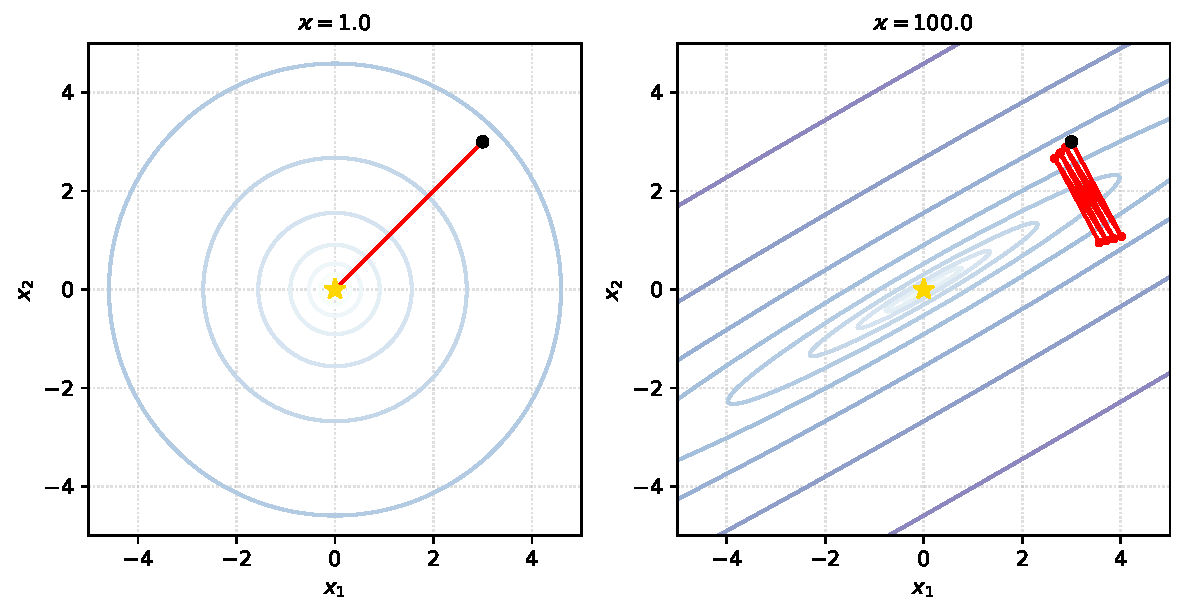
\includegraphics[keepaspectratio]{condition_number_gd.pdf}}}

\subsection{Ускорение из первых
принципов}\label{ux443ux441ux43aux43eux440ux435ux43dux438ux435-ux438ux437-ux43fux435ux440ux432ux44bux445-ux43fux440ux438ux43dux446ux438ux43fux43eux432}

\[
f(x) = \frac{1}{2} x^T A x - b^T x \qquad x_{k+1} = x_k - \alpha_k \nabla f(x_k).
\]

Пусть \(x^*\) будет единственным решением системы линейных уравнений
\(Ax=b\) и пусть \(e_k = x_k - x^*\), где
\(x_{k+1}=x_k - \alpha_k (Ax_k-b)\) определяется рекурсивно, начиная с
некоторого \(x_0\), а \(\alpha_k\) --- шаг, который мы определим позже.
\[
e_{k+1} = (I-\alpha_k A)e_k.
\]

\subsubsection{Полиномы}\label{ux43fux43eux43bux438ux43dux43eux43cux44b}

Вышеуказанный расчет дает нам \(e_k = p_k(A)e_0,\)

где \(p_k\) является полиномом \[
p_k(a) = \prod_{i=1}^k (1-\alpha_ia).
\]

Мы можем ограничить норму ошибки как \[
\|e_k\|\le \|p_k(A)\|\cdot\|e_0\|\,.
\]

Поскольку \(A\) является симметричной матрицей с собственными значениями
в \([\mu,L],\): \[
\|p_k(A)\|\le \max_{\mu\le a\le L} \left|p_k(a)\right|\,.
\] Это приводит к интересной постановке задачи: среди всех полиномов,
удовлетворяющих \(p_k(0)=1\), мы ищем полином, значение которого как
можно меньше отклоняется от нуля на интервале \([\mu,L]\).

\subsection{Наивное полиномиальное
решение}\label{ux43dux430ux438ux432ux43dux43eux435-ux43fux43eux43bux438ux43dux43eux43cux438ux430ux43bux44cux43dux43eux435-ux440ux435ux448ux435ux43dux438ux435}

Наивное решение состоит в том, чтобы выбрать равномерный шаг
\(\alpha_k=\frac{2}{\mu+L}\). Благодаря этому \(|p_k(\mu)| = |p_k(L)|\).
\[
\|e_k\|\le \left(\frac{\varkappa-1}{\varkappa+1}\right)^k\|e_0\|
\] Это точно та же скорость, которую мы доказали в предыдущей лекции для
любой гладкой и сильно выпуклой функции.

Давайте посмотрим на этот полином поближе. На правом рисунке мы выбираем
\(\mu=1\) и \(L=10\) так, что \(\varkappa=10\). Следовательно,
соответствующий интервал равен \([1,10]\).

Можем ли мы сделать лучше? Ответ --- да.

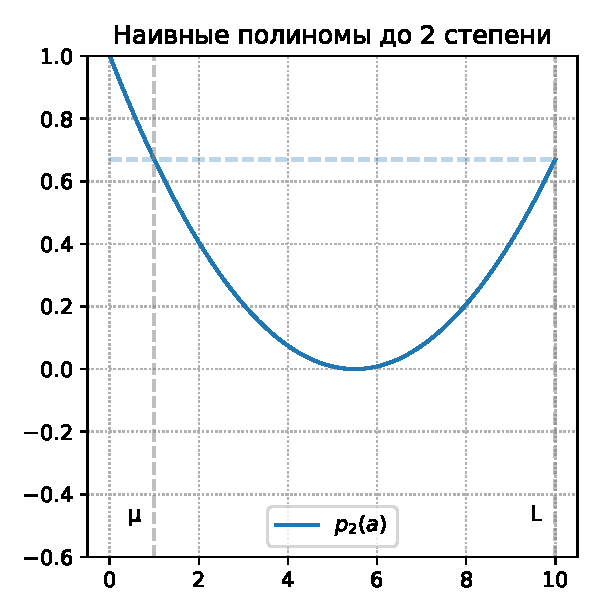
\includegraphics[width=0.5\columnwidth]{gd_polynom_2_ru.pdf}
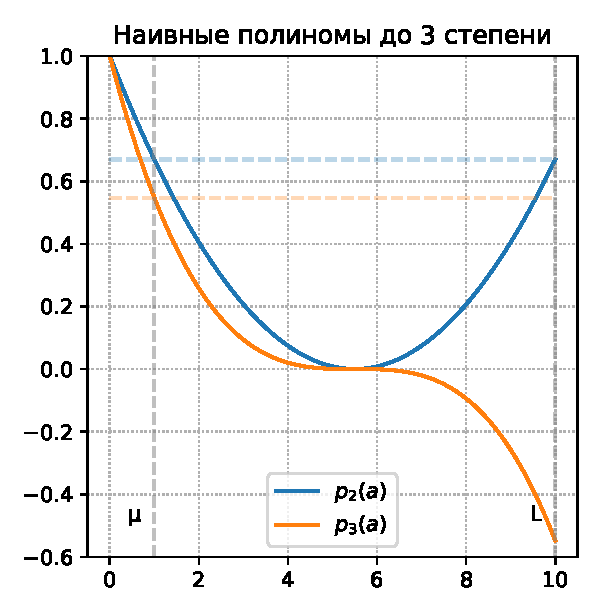
\includegraphics[width=0.5\columnwidth]{gd_polynom_3_ru.pdf}
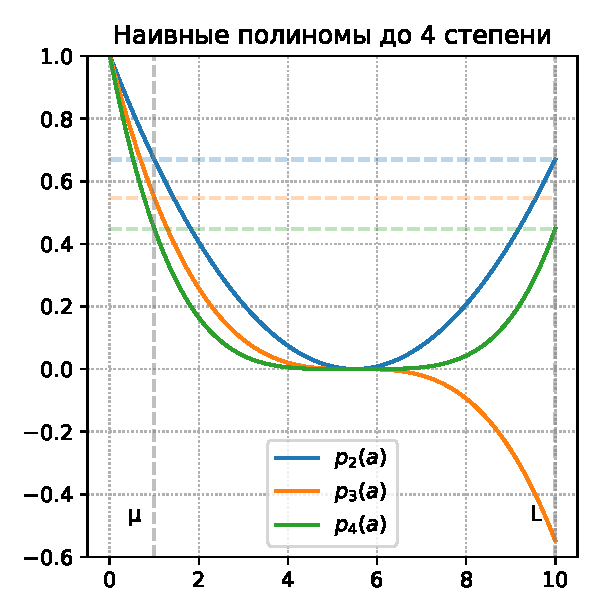
\includegraphics[width=0.5\columnwidth]{gd_polynom_4_ru.pdf}
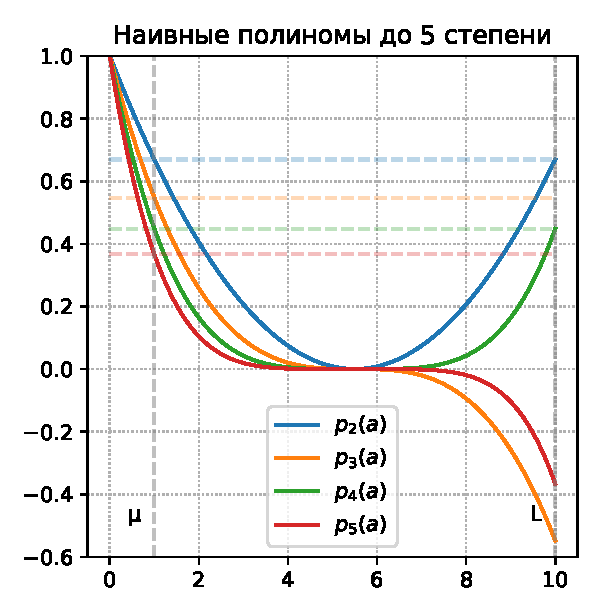
\includegraphics[width=0.5\columnwidth]{gd_polynom_5_ru.pdf}
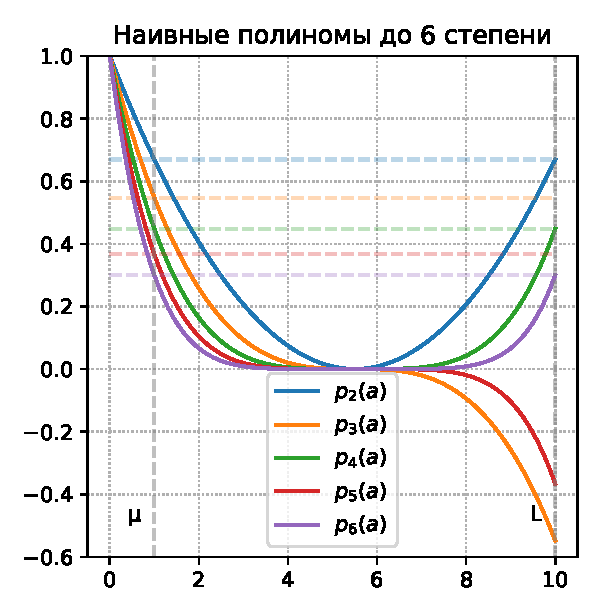
\includegraphics[width=0.5\columnwidth]{gd_polynom_6_ru.pdf}

\subsection{Полиномы
Чебышева}\label{ux43fux43eux43bux438ux43dux43eux43cux44b-ux447ux435ux431ux44bux448ux435ux432ux430}

Полиномы Чебышёва дают оптимальный ответ на поставленный вопрос. При
соответствующем шкалировании они минимизируют абсолютное значение на
заданном интервале \([\mu,L]\) , одновременно удовлетворяя
нормировочному условию \(p(0)=1\). \[
\begin{aligned}
T_0(x) &= 1\\
T_1(x) &= x\\
T_k(x) &=2xT_{k-1}(x)-T_{k-2}(x),\qquad k\ge 2.\\
\end{aligned}
\]

Давайте построим стандартные полиномы Чебышёва (без масштабирования):

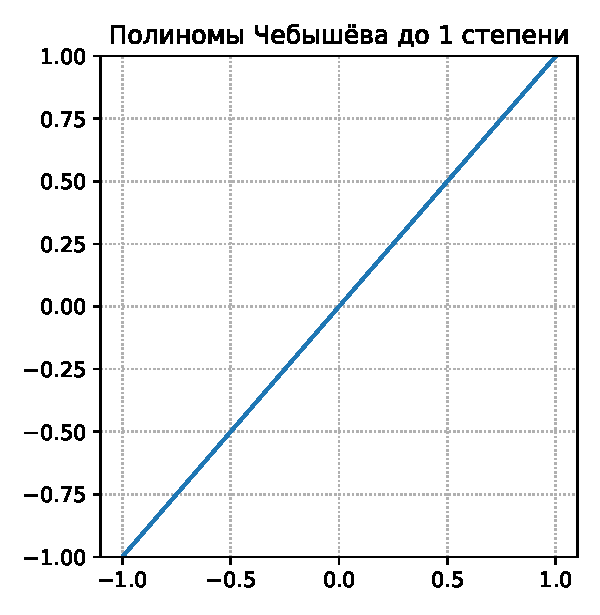
\includegraphics[width=0.5\columnwidth]{gd_polynom_cheb_1_ru.pdf}
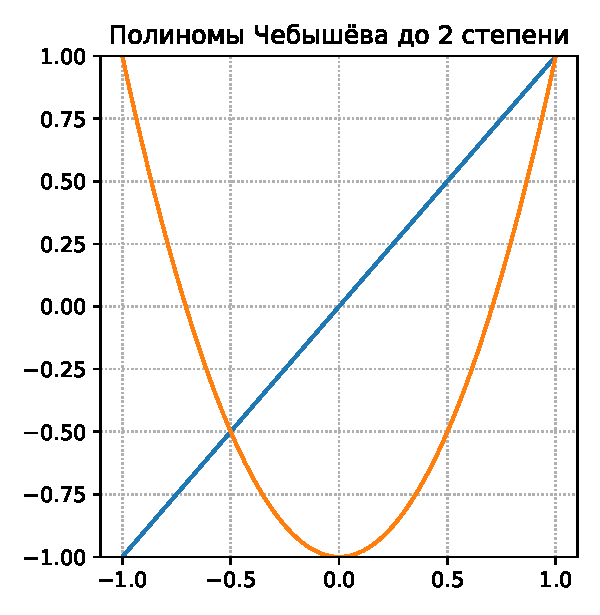
\includegraphics[width=0.5\columnwidth]{gd_polynom_cheb_2_ru.pdf}
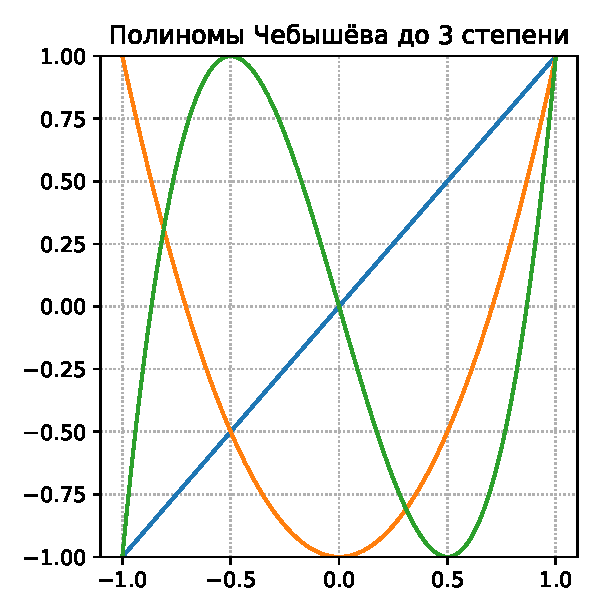
\includegraphics[width=0.5\columnwidth]{gd_polynom_cheb_3_ru.pdf}
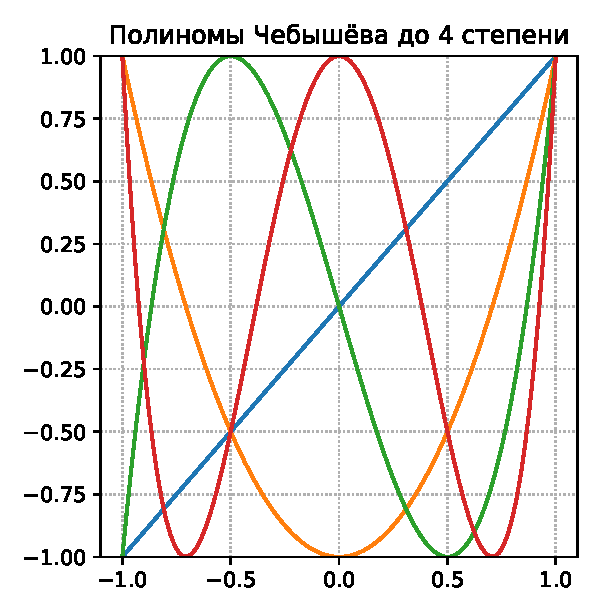
\includegraphics[width=0.5\columnwidth]{gd_polynom_cheb_4_ru.pdf}
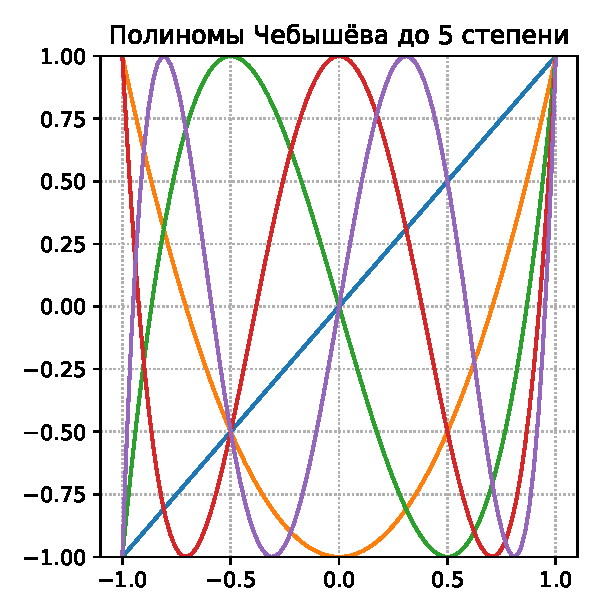
\includegraphics[width=0.5\columnwidth]{gd_polynom_cheb_5_ru.pdf}

\subsection{Отшкалированные полиномы
Чебышёва}\label{ux43eux442ux448ux43aux430ux43bux438ux440ux43eux432ux430ux43dux43dux44bux435-ux43fux43eux43bux438ux43dux43eux43cux44b-ux447ux435ux431ux44bux448ux451ux432ux430}

Оригинальные полиномы Чебышёва определены на интервале \([-1,1]\). Чтобы
использовать их для наших целей, мы должны отшкалировать их на интервал
\([\mu,L]\).

Мы будем использовать следующее аффинное преобразование: \[
x = \frac{L + \mu - 2a}{L - \mu}, \quad a \in [\mu,L], \quad x \in [-1,1]. 
\]

Обратите внимание, что \(x=1\) соответствует \(a=\mu\), \(x=-1\)
соответствует \(a=L\) и \(x=0\) соответствует \(a=\frac{\mu+L}{2}\). Это
преобразование гарантирует, что поведение полинома Чебышёва на интервале
\([-1,1]\) транслируется на интервал \([\mu, L]\).

В нашем анализе ошибок мы требуем, чтобы полином был равен 1 в 0 (т.е.
\(p_k(0)=1\)). После применения преобразования значение \(T_k\) в точке,
соответствующей \(a=0\), может не быть 1. Следовательно, мы умножаем на
обратную величину \(T_k\) в точке \[
\frac{L+\mu}{L-\mu}, \qquad \text{что обеспечивает} \qquad P_k(0)= T_k\left(\frac{L+\mu-0}{L-\mu}\right) \cdot T_k\left(\frac{L+\mu}{L-\mu}\right)^{-1} = 1.
\]

Построим отшкалированные полиномы Чебышёва \[
P_k(a) = T_k\left(\frac{L+\mu-2a}{L-\mu}\right) \cdot T_k\left(\frac{L+\mu}{L-\mu}\right)^{-1}
\] и увидим, что они больше подходят для нашей задачи, чем наивные
полиномы на интервале \([\mu,L]\).

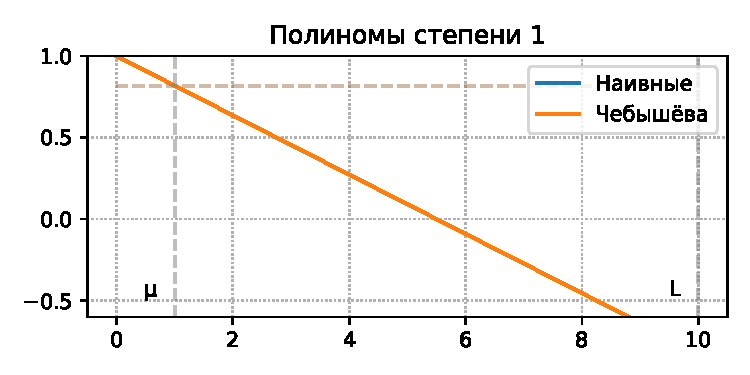
\includegraphics[width=0.5\columnwidth,height=0.8\textheight,keepaspectratio]{gd_polynoms_1_ru.pdf}
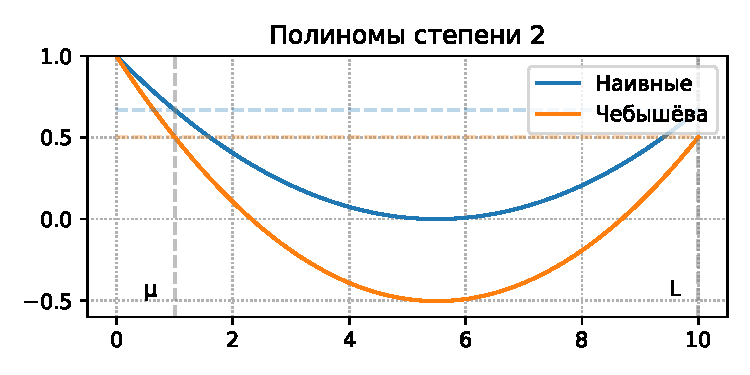
\includegraphics[width=0.5\columnwidth,height=0.8\textheight,keepaspectratio]{gd_polynoms_2_ru.pdf}
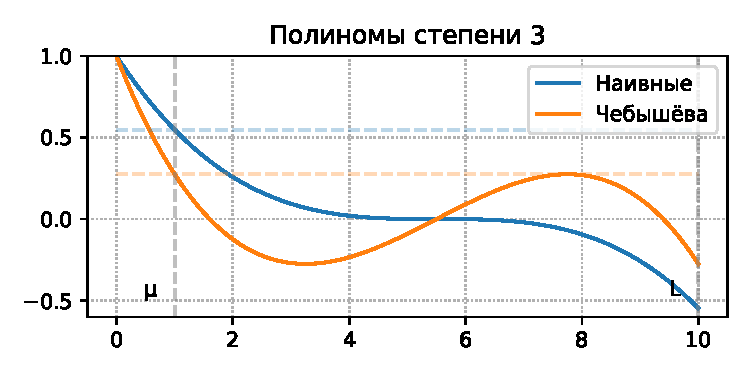
\includegraphics[width=0.5\columnwidth,height=0.8\textheight,keepaspectratio]{gd_polynoms_3_ru.pdf}
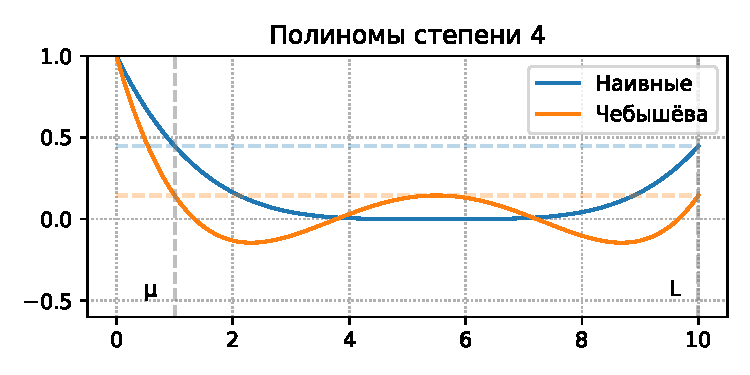
\includegraphics[width=0.5\columnwidth,height=0.8\textheight,keepaspectratio]{gd_polynoms_4_ru.pdf}
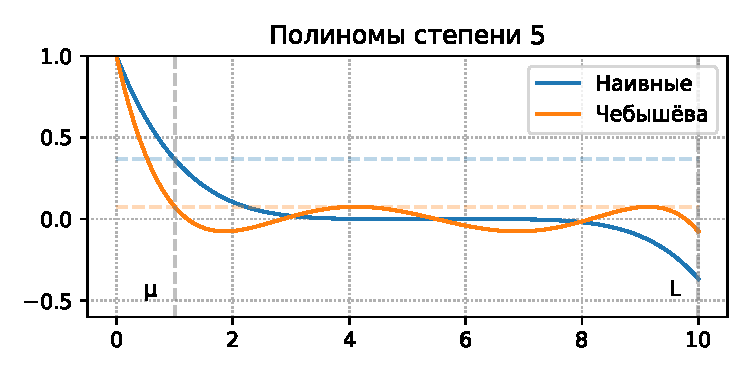
\includegraphics[width=0.5\columnwidth,height=0.8\textheight,keepaspectratio]{gd_polynoms_5_ru.pdf}
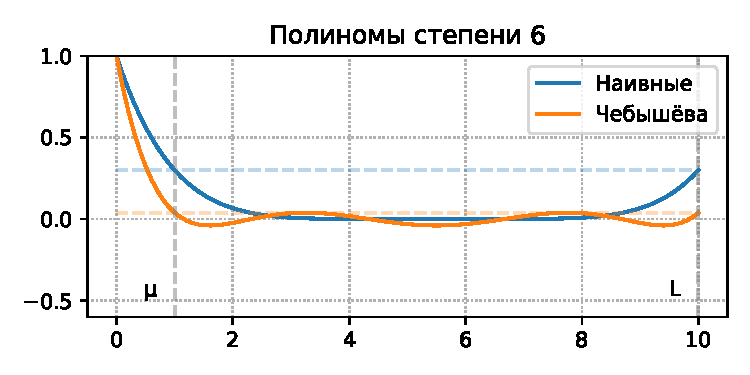
\includegraphics[width=0.5\columnwidth,height=0.8\textheight,keepaspectratio]{gd_polynoms_6_ru.pdf}
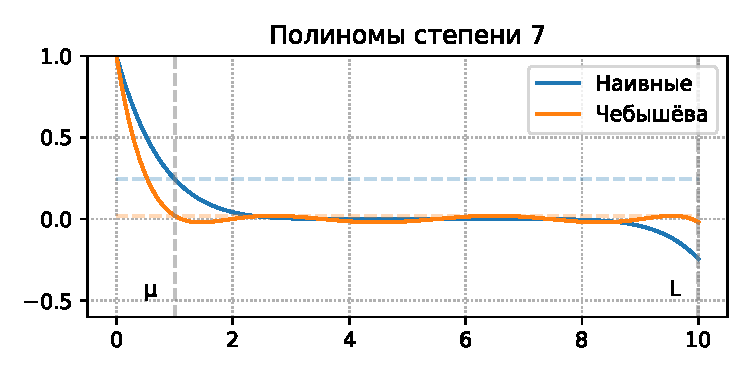
\includegraphics[width=0.5\columnwidth,height=0.8\textheight,keepaspectratio]{gd_polynoms_7_ru.pdf}
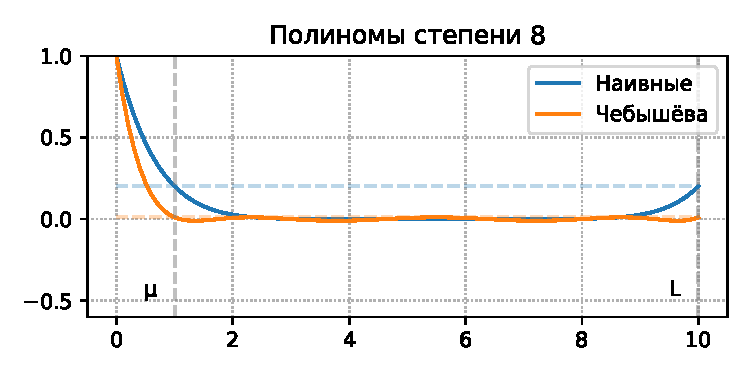
\includegraphics[width=0.5\columnwidth,height=0.8\textheight,keepaspectratio]{gd_polynoms_8_ru.pdf}
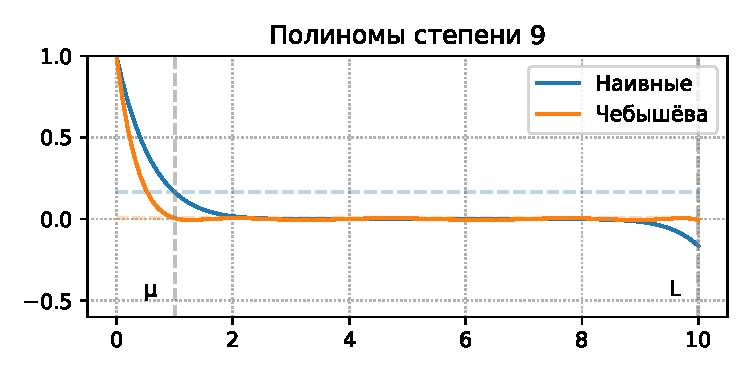
\includegraphics[width=0.5\columnwidth,height=0.8\textheight,keepaspectratio]{gd_polynoms_9_ru.pdf}
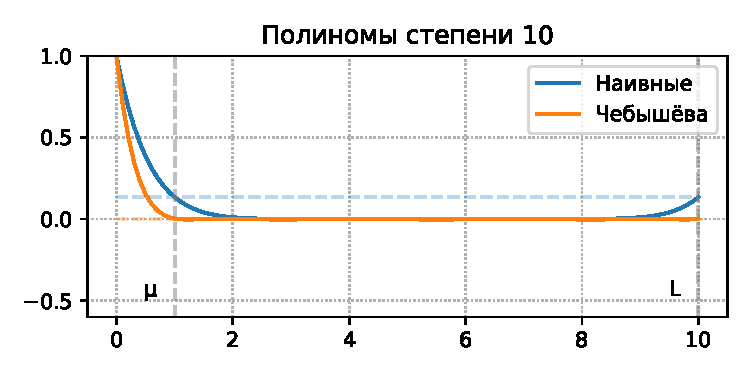
\includegraphics[width=0.5\columnwidth,height=0.8\textheight,keepaspectratio]{gd_polynoms_10_ru.pdf}

\subsection{Верхняя оценка для полиномов
Чебышёва}\label{ux432ux435ux440ux445ux43dux44fux44f-ux43eux446ux435ux43dux43aux430-ux434ux43bux44f-ux43fux43eux43bux438ux43dux43eux43cux43eux432-ux447ux435ux431ux44bux448ux451ux432ux430}

Мы можем видеть, что максимальное значение полинома Чебышёва на
интервале \([\mu,L]\) достигается на концах отрезка в точках \(a=\mu\) и
\(a=L\). Следовательно, мы можем использовать следующую верхнюю оценку:
\[
\|P_k(A)\|_2 \le P_k(\mu) = T_k\left(\frac{L+\mu-2\mu}{L-\mu}\right) \cdot T_k\left(\frac{L+\mu}{L-\mu}\right)^{-1} = T_k\left(1\right) \cdot T_k\left(\frac{L+\mu}{L-\mu}\right)^{-1} = T_k\left(\frac{L+\mu}{L-\mu}\right)^{-1}
\]

Используя определение числа обусловленности
\(\varkappa = \frac{L}{\mu}\), мы получаем: \[
\|P_k(A)\|_2 \le T_k\left(\frac{\varkappa+1}{\varkappa-1}\right)^{-1} = T_k\left(1 + \frac{2}{\varkappa-1}\right)^{-1} = T_k\left(1 + \epsilon\right)^{-1}, \quad \epsilon = \frac{2}{\varkappa-1}.
\]

Именно в этот момент явно возникнет ускорение. Мы ограничим значение
\(\|P_k(A)\|_2\) сверху величиной
\(\left(\frac{1}{1 + \sqrt{\epsilon}}\right)^k\). Для этого детально
изучим величину \(|T_k(1 + \epsilon)|\).

Чтобы ограничить \(|P_k|\) сверху, мы должны ограничить
\(|T_k(1 + \epsilon)|\) снизу.

\begin{enumerate}
\def\labelenumi{\arabic{enumi}.}
\item
  Для любого \(x\ge 1\), полиномы Чебышёва первого рода могут быть
  записаны как \[
  \begin{aligned}
  T_k(x)&=\cosh\left(k\,\mathrm{arccosh}(x)\right)\\
  T_k(1+\epsilon)&=\cosh\left(k\,\mathrm{arccosh}(1+\epsilon)\right).
  \end{aligned}
  \]
\item
  Помните, что: \[
   \cosh(x)=\frac{e^x+e^{-x}}{2} \quad \mathrm{arccosh}(x) = \ln(x + \sqrt{x^2-1}).
   \]
\item
  Теперь, пусть \(\phi=\mathrm{arccosh}(1+\epsilon)\), \[
   e^{\phi}=1+\epsilon + \sqrt{2\epsilon+\epsilon^2} \geq 1+\sqrt{\epsilon}.
   \]
\end{enumerate}

\begin{enumerate}
\def\labelenumi{\arabic{enumi}.}
\setcounter{enumi}{3}
\item
  Следовательно, \[
   \begin{aligned}
   T_k(1+\epsilon)&=\cosh\left(k\,\mathrm{arccosh}(1+\epsilon)\right) \\
   &= \cosh\left(k\phi\right) \\
   &= \frac{e^{k\phi} + e^{-k\phi}}{2} \geq\frac{e^{k\phi}}{2} \\
   &= \frac{\left(1+\sqrt{\epsilon}\right)^k}{2}.
   \end{aligned}
   \]
\item
  Наконец, мы получаем: \[
   \begin{aligned}
   \|e_k\| &\leq \|P_k(A)\| \|e_0\| \leq \frac{2}{\left(1 + \sqrt{\epsilon}\right)^k} \|e_0\| \\ 
   &\leq 2 \left(1 + \sqrt{\frac{2}{\varkappa-1}}\right)^{-k} \|e_0\| \\
   &\leq 2 \exp\left( - \sqrt{\frac{2}{\varkappa-1}} k\right) \|e_0\|
   \end{aligned}
   \]
\end{enumerate}

\subsection{Ускоренный метод
{[}1/2{]}}\label{ux443ux441ux43aux43eux440ux435ux43dux43dux44bux439-ux43cux435ux442ux43eux434-12}

Из-за рекурсивного определения полиномов Чебышёва мы непосредственно
получаем итерационную схему ускоренного алгоритма. Переформулируя
рекурсию в терминах наших отшкалированных полиномов Чебышёва, мы
получаем: \[
T_{k+1}(x) =2xT_{k}(x)-T_{k-1}(x)
\]

Принимая во внимание, что \(x = \frac{L+\mu-2a}{L-\mu}\), и:

\[
\begin{aligned}
P_k(a) &= T_k\left(\frac{L+\mu-2a}{L-\mu}\right) T_k\left(\frac{L+\mu}{L-\mu}\right)^{-1}  \\
T_k\left(\frac{L+\mu-2a}{L-\mu}\right) &= P_k(a) T_k\left(\frac{L+\mu}{L-\mu}\right) 
\end{aligned}
\]

\[
\begin{aligned}
T_{k-1}\left(\frac{L+\mu-2a}{L-\mu}\right) &= P_{k-1}(a) T_{k-1}\left(\frac{L+\mu}{L-\mu}\right) \\
T_{k+1}\left(\frac{L+\mu-2a}{L-\mu}\right) &= P_{k+1}(a) T_{k+1}\left(\frac{L+\mu}{L-\mu}\right)
\end{aligned}
\]

\[
\begin{aligned}
P_{k+1}(a) t_{k+1} &= 2 \frac{L+\mu-2a}{L-\mu} P_{k}(a) t_{k} - P_{k-1}(a) t_{k-1} \text{, где } t_{k} = T_{k}\left(\frac{L+\mu}{L-\mu}\right) \\
P_{k+1}(a) &= 2 \frac{L+\mu-2a}{L-\mu} P_{k}(a) \frac{t_{k}}{t_{k+1}} - P_{k-1}(a) \frac{t_{k-1}}{t_{k+1}}
\end{aligned}
\]

Поскольку мы имеем \(P_{k+1}(0) = P_{k}(0) = P_{k-1}(0) = 1\), получаем
рекуррентную формулу вида: \[
P_{k+1}(a) = (1 - \alpha_k a) P_k(a) + \beta_k \left(P_{k}(a) - P_{k-1}(a) \right).
\]

\subsection{Ускоренный метод
{[}2/2{]}}\label{ux443ux441ux43aux43eux440ux435ux43dux43dux44bux439-ux43cux435ux442ux43eux434-22}

Перегруппируя члены, мы получаем: \[
\begin{aligned}
P_{k+1}(a) &= (1 + \beta_k) P_k(a) - \alpha_k a P_k(a) - \beta_k P_{k-1}(a), \\
P_{k+1}(a) &= 2 \frac{L+\mu}{L-\mu}  \frac{t_{k}}{t_{k+1}} P_{k}(a) - \frac{4a}{L-\mu}  \frac{t_{k}}{t_{k+1}}P_{k}(a) - \frac{t_{k-1}}{t_{k+1}} P_{k-1}(a)
\end{aligned}
\]

\[
\begin{cases}
\beta_k = \dfrac{t_{k-1}}{t_{k+1}}, \\[6pt]
\alpha_k = \dfrac{4}{L-\mu} \dfrac{t_k}{t_{k+1}}, \\[6pt]
1 + \beta_k = 2 \dfrac{L + \mu}{L - \mu} \dfrac{t_k}{t_{k+1}}
\end{cases}
\]

Мы почти закончили :) Помним, что \(e_{k+1} = P_{k+1}(A) e_0\). Также
обратим внимание, что мы работаем с квадратичной задачей, поэтому мы
можем предположить \(x^* = 0\) без ограничения общности. В этом случае
\(e_0 = x_0\) и \(e_{k+1} = x_{k+1}\). \textbackslash{} \[
\begin{aligned}
x_{k+1} &= P_{k+1}(A) x_0 =  (I - \alpha_k A) P_k(A) x_0 + \beta_k \left(P_{k}(A) - P_{k-1}(A) \right) x_0 \\
&= (I - \alpha_k A) x_k + \beta_k \left(x_k - x_{k-1}\right)
\end{aligned}
\]

Для квадратичной задачи мы имеем \(\nabla f(x_k) = A x_k\), поэтому мы
можем переписать обновление как: \[
\boxed{
x_{k+1} = x_k - \alpha_k \nabla f(x_k) + \beta_k \left(x_k - x_{k-1}\right)
}
\]

\subsection{Ускорение из первых
принципов}\label{ux443ux441ux43aux43eux440ux435ux43dux438ux435-ux438ux437-ux43fux435ux440ux432ux44bux445-ux43fux440ux438ux43dux446ux438ux43fux43eux432-1}

\href{https://fmin.xyz/docs/visualizations/chebyshev_gd.mp4}{\pandocbounded{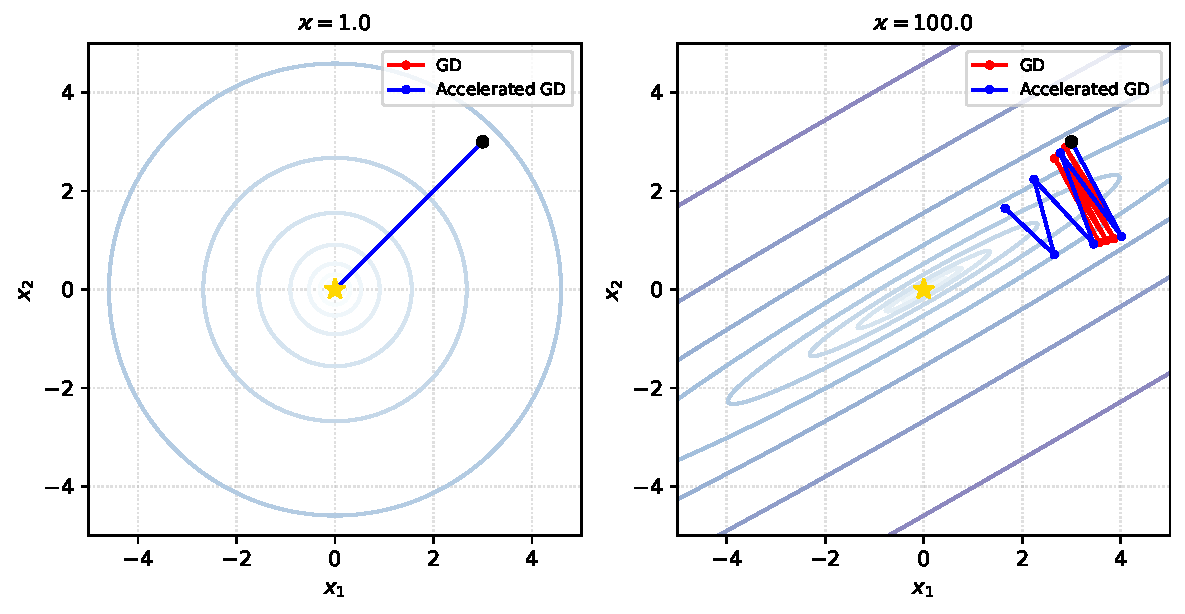
\includegraphics[keepaspectratio]{chebyshev_gd.pdf}}}

\section{Метод тяжёлого
шарика}\label{ux43cux435ux442ux43eux434-ux442ux44fux436ux451ux43bux43eux433ux43e-ux448ux430ux440ux438ux43aux430}

\subsection{\texorpdfstring{\href{https://colab.research.google.com/github/MerkulovDaniil/optim/blob/master/assets/Notebooks/GD.ipynb}{Колебания
и
ускорение}}{Колебания и ускорение}}\label{ux43aux43eux43bux435ux431ux430ux43dux438ux44f-ux438-ux443ux441ux43aux43eux440ux435ux43dux438ux435}

\pandocbounded{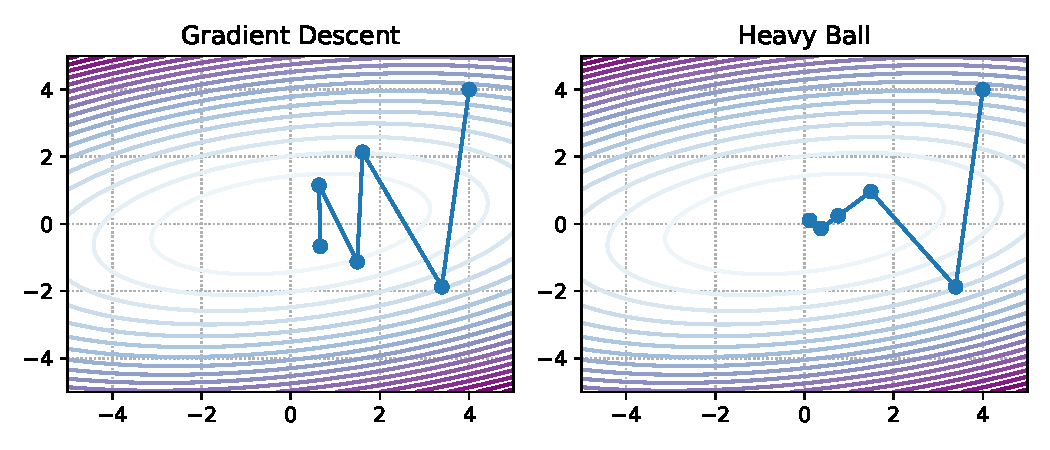
\includegraphics[keepaspectratio]{GD_vs_HB_hor.pdf}}

\subsection{Метод тяжёлого шарика
Поляка}\label{ux43cux435ux442ux43eux434-ux442ux44fux436ux451ux43bux43eux433ux43e-ux448ux430ux440ux438ux43aux430-ux43fux43eux43bux44fux43aux430}

\pandocbounded{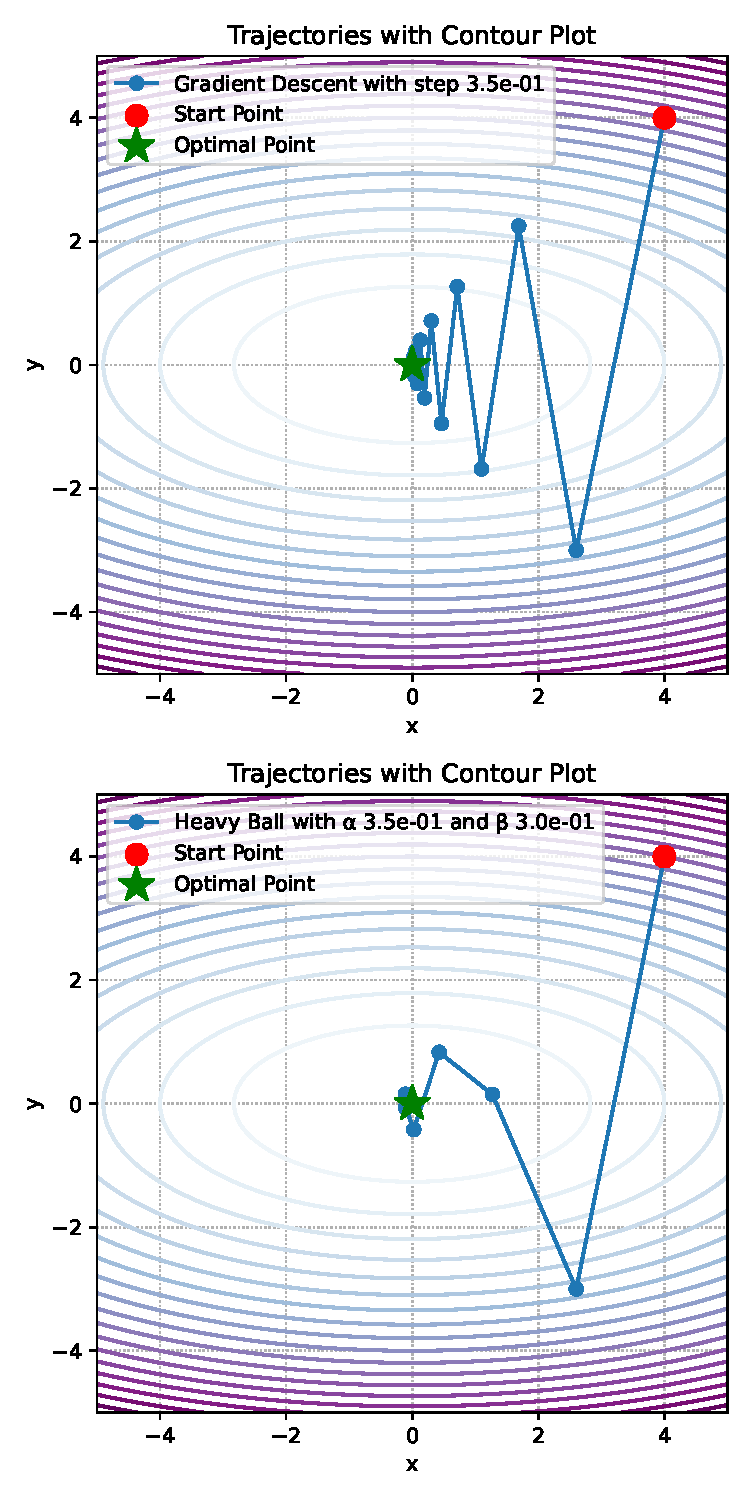
\includegraphics[keepaspectratio]{GD_HB.pdf}}

Давайте представим идею моментума (импульса, тяжёлого шарика),
предложенную Б.Т. Поляком в 1964 году. Обновление метода тяжёлого шарика
имеет вид

\[
x_{k+1} = x_k - \alpha \nabla f(x_k) + \beta (x_k - x_{k-1}).
\]

В нашем (квадратичном) случае это \[
\hat{x}_{k+1} = \hat{x}_k - \alpha \Lambda \hat{x}_k + \beta (\hat{x}_k - \hat{x}_{k-1}) = (I - \alpha \Lambda + \beta I) \hat{x}_k - \beta \hat{x}_{k-1}
\]

Это можно переписать как

\[
\begin{split}
&\hat{x}_{k+1} = (I - \alpha \Lambda + \beta I) \hat{x}_k - \beta \hat{x}_{k-1}, \\
&\hat{x}_{k} = \hat{x}_k.
\end{split}
\]

Давайте введем следующее обозначение: \(\hat{z}_k = \begin{bmatrix}
\hat{x}_{k+1} \\
\hat{x}_{k}
\end{bmatrix}\). Следовательно, \(\hat{z}_{k+1} = M \hat{z}_k\), где
матрица итерации \(M\) имеет вид:

\[
M = \begin{bmatrix} 
I - \alpha \Lambda + \beta I & - \beta I \\
I & 0_{d}
\end{bmatrix}.
\]

\subsection{Сведение к скалярному
случаю}\label{ux441ux432ux435ux434ux435ux43dux438ux435-ux43a-ux441ux43aux430ux43bux44fux440ux43dux43eux43cux443-ux441ux43bux443ux447ux430ux44e}

Обратим внимание, что \(M\) является матрицей \(2d \times 2d\) с
четырьмя блочно-диагональными матрицами размера \(d \times d\) внутри.
Это означает, что мы можем изменить порядок координат, чтобы сделать
\(M\) блочно-диагональной. Обратите внимание, что в уравнении ниже
матрица \(M\) обозначает то же самое, что и в обозначении выше, за
исключением описанной перестановки строк и столбцов. Мы используем эту
небольшую перегрузку обозначений для простоты.

\begin{figure}[H]

{\centering \pandocbounded{
\includegraphics[keepaspectratio]{Rearranging_squares.pdf}}

}

\caption{Иллюстрация перестановки матрицы \(M\)}

\end{figure}%

\[
\begin{aligned}
\begin{bmatrix} 
\hat{x}_{k}^{(1)} \\
\vdots \\
\hat{x}_{k}^{(d)} \\
\addlinespace 
\hat{x}_{k-1}^{(1)} \\
\vdots \\
\hat{x}_{k-1}^{(d)}
\end{bmatrix} \to 
\begin{bmatrix} 
\hat{x}_{k}^{(1)} \\
\addlinespace 
\hat{x}_{k-1}^{(1)} \\
\vdots \\
\hat{x}_{k}^{(d)} \\
\addlinespace 
\hat{x}_{k-1}^{(d)}
\end{bmatrix} \quad M = \begin{bmatrix}
M_1\\
&M_2\\
&&\ldots\\
&&&M_d
\end{bmatrix}
\end{aligned}
\]

где \(\hat{x}_{k}^{(i)}\) является \(i\)-й координатой вектора
\(\hat{x}_{k} \in \mathbb{R}^d\) и \(M_i\) обозначает \(2 \times 2\)
матрицу. Переупорядочение позволяет нам исследовать динамику метода
независимо от размерности. Асимптотическая скорость сходимости
\(2d\)-мерной последовательности векторов \(\hat{z}_k\) определяется
наихудшей скоростью сходимости среди его блока координат. Следовательно,
достаточно исследовать оптимизацию в одномерном случае.

Для \(i\)-й координаты, где \(\lambda_i\) --- \(i\)-е собственное
значение матрицы \(A\), имеем:

\[
M_i = \begin{bmatrix} 
1 - \alpha \lambda_i + \beta & -\beta \\
1 & 0
\end{bmatrix}.
\]

Метод будет сходиться, если \(\rho(M) < 1\), и оптимальные параметры
могут быть вычислены путем оптимизации спектрального радиуса \[
\alpha^*, \beta^* = \arg \min_{\alpha, \beta} \max_{i} \rho(M_i), \quad \alpha^* = \dfrac{4}{(\sqrt{L} + \sqrt{\mu})^2}, \quad \beta^* = \left(\dfrac{\sqrt{L} - \sqrt{\mu}}{\sqrt{L} + \sqrt{\mu}}\right)^2.
\]

Можно показать, что для таких параметров матрица \(M\) имеет комплексные
собственные значения, которые образуют комплексно-сопряжённую пару,
поэтому расстояние до оптимума (в этом случае \(\| z_k \|\)) обычно не
убывает монотонно.

\subsection{Сходимость метода тяжёлого шарика для квадратичной
функции}\label{ux441ux445ux43eux434ux438ux43cux43eux441ux442ux44c-ux43cux435ux442ux43eux434ux430-ux442ux44fux436ux451ux43bux43eux433ux43e-ux448ux430ux440ux438ux43aux430-ux434ux43bux44f-ux43aux432ux430ux434ux440ux430ux442ux438ux447ux43dux43eux439-ux444ux443ux43dux43aux446ux438ux438}

Мы можем явно вычислить собственные значения \(M_i\):

\[
\lambda^M_1, \lambda^M_2 = \lambda \left( \begin{bmatrix} 
1 - \alpha \lambda_i + \beta & -\beta \\
1 & 0
\end{bmatrix}\right) = \dfrac{1+\beta - \alpha \lambda_i \pm \sqrt{(1+\beta - \alpha\lambda_i)^2 - 4\beta}}{2}.
\]

Когда \(\alpha\) и \(\beta\) оптимальны (\(\alpha^*, \beta^*\)),
собственные значения являются комплексно-сопряженной парой
\((1+\beta - \alpha\lambda_i)^2 - 4\beta \leq 0\), т.е.
\(\beta \geq (1 - \sqrt{\alpha \lambda_i})^2\).

\[
\text{Re}(\lambda^M) = \dfrac{L + \mu - 2\lambda_i}{(\sqrt{L} + \sqrt{\mu})^2}, \quad \text{Im}(\lambda^M) = \dfrac{\pm 2\sqrt{(L - \lambda_i)(\lambda_i - \mu)}}{(\sqrt{L} + \sqrt{\mu})^2}, \quad \lvert \lambda^M \rvert = \dfrac{L - \mu}{(\sqrt{L} + \sqrt{\mu})^2}.
\]

И скорость сходимости не зависит от шага и равна \(\sqrt{\beta^*}\).

\begin{tcolorbox}[enhanced jigsaw, rightrule=.15mm, coltitle=black, title=\textcolor{quarto-callout-color}{\faInfo}\hspace{0.5em}{Theorem}, colbacktitle=quarto-callout-color!10!white, opacityback=0, colframe=quarto-callout-color-frame, bottomtitle=1mm, toptitle=1mm, titlerule=0mm, arc=.35mm, leftrule=.75mm, breakable, toprule=.15mm, bottomrule=.15mm, opacitybacktitle=0.6, left=2mm, colback=white]

Предположим, что \(f\) является \(\mu\)-сильно выпуклой и \(L\)-гладкой
квадратичной функцией. Тогда метод тяжёлого шарика с параметрами \[
\alpha = \dfrac{4}{(\sqrt{L} + \sqrt{\mu})^2}, \beta = \left(\dfrac{\sqrt{L} - \sqrt{\mu}}{\sqrt{L} + \sqrt{\mu}}\right)^2
\]

сходится линейно:

\[
\|x_k - x^*\|_2 \leq \left( \dfrac{\sqrt{\varkappa} - 1}{\sqrt{\varkappa} + 1} \right)^k \|x_0 - x^*\|
\]

\end{tcolorbox}

\subsection[Глобальная сходимость метода тяжёлого шарика
]{\texorpdfstring{Глобальная сходимость метода тяжёлого шарика
\footnote{\href{https://arxiv.org/abs/1412.7457}{Глобальная сходимость
  метода тяжёлого шарика для выпуклой оптимизации, Euhanna Ghadimi et
  al.}}}{Глобальная сходимость метода тяжёлого шарика }}\label{ux433ux43bux43eux431ux430ux43bux44cux43dux430ux44f-ux441ux445ux43eux434ux438ux43cux43eux441ux442ux44c-ux43cux435ux442ux43eux434ux430-ux442ux44fux436ux451ux43bux43eux433ux43e-ux448ux430ux440ux438ux43aux430}

\begin{tcolorbox}[enhanced jigsaw, rightrule=.15mm, coltitle=black, title=\textcolor{quarto-callout-color}{\faInfo}\hspace{0.5em}{Theorem}, colbacktitle=quarto-callout-color!10!white, opacityback=0, colframe=quarto-callout-color-frame, bottomtitle=1mm, toptitle=1mm, titlerule=0mm, arc=.35mm, leftrule=.75mm, breakable, toprule=.15mm, bottomrule=.15mm, opacitybacktitle=0.6, left=2mm, colback=white]

Предположим, что \(f\) является гладкой и выпуклой и что

\[
\beta\in[0,1),\quad \alpha\in\biggl(0,\dfrac{2(1-\beta)}{L}\biggr).
\]

Тогда последовательность \(\{x_k\}\), генерируемая итерациями тяжёлого
шарика, удовлетворяет

\[
f(\overline{x}_T)-f^{\star} \leq  \left\{
\begin{array}[l]{ll}
\frac{\Vert x_{0}-x^\star\Vert^2}{2(T+1)}\biggl(\frac{L\beta}{1-\beta}+\frac{1-\beta}{\alpha}\biggr),\;\;\textup{if}\;\;
\alpha\in\bigl(0,\dfrac{1-\beta}{L}\bigr],\\
\frac{\Vert x_{0}-x^\star\Vert^2}{2(T+1)(2(1-\beta)-\alpha L)}\biggl({L\beta}+\frac{(1-\beta)^2}{\alpha}\biggr),\;\;\textup{if}\;\;
\alpha\in\bigl[\dfrac{1-\beta}{L},\dfrac{2(1-\beta)}{L}\bigr),
\end{array}
\right.
\]

где \(\overline{x}_T\) среднее Чезаро последовательности итераций, т.е.

\[
\overline{x}_T = \frac{1}{T+1}\sum_{k=0}^T x_k.
\]

\end{tcolorbox}

\begin{tcolorbox}[enhanced jigsaw, rightrule=.15mm, coltitle=black, title=\textcolor{quarto-callout-color}{\faInfo}\hspace{0.5em}{Theorem}, colbacktitle=quarto-callout-color!10!white, opacityback=0, colframe=quarto-callout-color-frame, bottomtitle=1mm, toptitle=1mm, titlerule=0mm, arc=.35mm, leftrule=.75mm, breakable, toprule=.15mm, bottomrule=.15mm, opacitybacktitle=0.6, left=2mm, colback=white]

Предположим, что \(f\) является гладкой и сильно выпуклой и что

\[
\alpha\in\biggl(0,\dfrac{2}{L}\biggr),\quad 0\leq  \beta<\dfrac{1}{2}\biggl( \dfrac{\mu \alpha}{2}+\sqrt{\dfrac{\mu^2\alpha^2}{4}+4(1-\frac{\alpha L}{2})} \biggr) .
\]

Тогда последовательность \(\{x_k\}\), генерируемая итерациями
методатяжёлого шарика, сходится линейно к единственному оптимальному
решению \(x^\star\). В частности,

\[
f(x_{k})-f^\star \leq q^k (f(x_0)-f^\star),
\]

где \(q\in[0,1)\).

\end{tcolorbox}

\subsection{Итоги по методу тяжёлого
шарика}\label{ux438ux442ux43eux433ux438-ux43fux43e-ux43cux435ux442ux43eux434ux443-ux442ux44fux436ux451ux43bux43eux433ux43e-ux448ux430ux440ux438ux43aux430}

\begin{itemize}
\tightlist
\item
  Обеспечивает ускоренную сходимость для сильно выпуклых квадратичных
  задач.
\item
  Локально ускоренная сходимость была доказана в оригинальной статье.
\item
  Недавно \footnote{\href{https://arxiv.org/pdf/2307.11291}{Provable
    non-accelerations of the heavy-ball method}} было доказано, что
  глобального ускорения сходимости для метода не существует.
\item
  Метод не был чрезвычайно популярен до ML-бума.
\item
  Сейчас он фактически является стандартом для практического ускорения
  методов градиентного спуска, в том числе для невыпуклых задач
  (обучение нейронных сетей).
\end{itemize}

\section{Ускоренный градиентный метод
Нестерова}\label{ux443ux441ux43aux43eux440ux435ux43dux43dux44bux439-ux433ux440ux430ux434ux438ux435ux43dux442ux43dux44bux439-ux43cux435ux442ux43eux434-ux43dux435ux441ux442ux435ux440ux43eux432ux430}

\subsection{Концепция ускоренного градиентного метода
Нестерова}\label{ux43aux43eux43dux446ux435ux43fux446ux438ux44f-ux443ux441ux43aux43eux440ux435ux43dux43dux43eux433ux43e-ux433ux440ux430ux434ux438ux435ux43dux442ux43dux43eux433ux43e-ux43cux435ux442ux43eux434ux430-ux43dux435ux441ux442ux435ux440ux43eux432ux430}

\[
x_{k+1} = x_k - \alpha \nabla f(x_k)
\]

\[
x_{k+1} = x_k - \alpha \nabla f(x_k) + \beta (x_k - x_{k-1})
\]

\[
\begin{cases}y_{k+1} = x_k + \beta (x_k - x_{k-1}) \\ x_{k+1} = y_{k+1} - \alpha \nabla f(y_{k+1}) \end{cases}
\]

Давайте определим следующие обозначения

\[
\begin{aligned}
x^+ &= x - \alpha \nabla f(x) \qquad &\text{Градиентный шаг} \\
d_k &= \beta_k (x_k - x_{k-1}) \qquad &\text{Импульс}
\end{aligned}
\]

Тогда мы можем записать:

\[
\begin{aligned}
x_{k+1} &= x_k^+ \qquad &\text{Градиентный спуск} \\
x_{k+1} &= x_k^+ + d_k \qquad &\text{Метод тяжёлого шарика} \\
x_{k+1} &= (x_k + d_k)^+ \qquad &\text{Ускоренный градиентный метод Нестерова}
\end{aligned}
\]

\centering

\pandocbounded{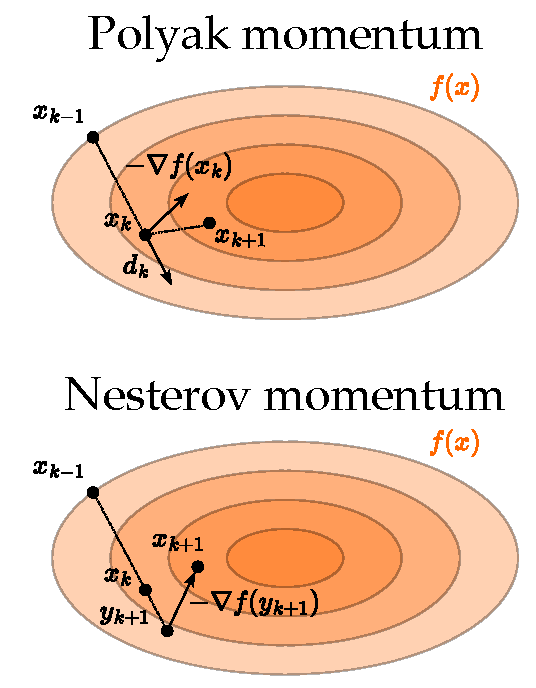
\includegraphics[keepaspectratio]{AGD.pdf}}

\subsection{Сходимость для выпуклых
функций}\label{ux441ux445ux43eux434ux438ux43cux43eux441ux442ux44c-ux434ux43bux44f-ux432ux44bux43fux443ux43aux43bux44bux445-ux444ux443ux43dux43aux446ux438ux439}

\begin{tcolorbox}[enhanced jigsaw, rightrule=.15mm, coltitle=black, title=\textcolor{quarto-callout-color}{\faInfo}\hspace{0.5em}{Theorem}, colbacktitle=quarto-callout-color!10!white, opacityback=0, colframe=quarto-callout-color-frame, bottomtitle=1mm, toptitle=1mm, titlerule=0mm, arc=.35mm, leftrule=.75mm, breakable, toprule=.15mm, bottomrule=.15mm, opacitybacktitle=0.6, left=2mm, colback=white]

Предположим, что \(f : \mathbb{R}^n \rightarrow \mathbb{R}\) является
выпуклой и \(L\)-гладкой. Ускоренный градиентный метод Нестерова (NAG)
предназначен для решения задачи минимизации, начиная с начальной точки
\(x_0 = y_0 \in \mathbb{R}^n\) и \(\lambda_0 = 0\). Алгоритм выполняет
следующие шаги: \[
\begin{aligned}
&\textbf{Обновление градиента: } &x_{k+1} &= y_k - \frac{1}{L} \nabla f(y_k) \\
& \textbf{Вес экстраполяции: } &\lambda_{k+1} &= \frac{1 + \sqrt{1 + 4\lambda_k^2}}{2} \\
& \quad &\gamma_k &= \frac{\lambda_k - 1}{\lambda_{k+1}} \\
&\textbf{Экстраполяция: } &y_{k+1} &= x_{k+1} + \gamma_k\left(x_{k+1} - x_k\right)
\end{aligned}
\] Последовательность \(\{f(x_k)\}_{k\in\mathbb{N}}\), генерируемая
алгоритмом, сходится к оптимальному значению \(f^*\) со скоростью
\(\mathcal{O}\left(\frac{1}{k^2}\right)\), в частности: \[
f(x_k) - f^* \leq \frac{2L \|x_0 - x^*\|^2}{k^2}
\]

\end{tcolorbox}

\subsection{Ускоренная сходимость для сильно выпуклых
функций}\label{ux443ux441ux43aux43eux440ux435ux43dux43dux430ux44f-ux441ux445ux43eux434ux438ux43cux43eux441ux442ux44c-ux434ux43bux44f-ux441ux438ux43bux44cux43dux43e-ux432ux44bux43fux443ux43aux43bux44bux445-ux444ux443ux43dux43aux446ux438ux439}

\begin{tcolorbox}[enhanced jigsaw, rightrule=.15mm, coltitle=black, title=\textcolor{quarto-callout-color}{\faInfo}\hspace{0.5em}{Theorem}, colbacktitle=quarto-callout-color!10!white, opacityback=0, colframe=quarto-callout-color-frame, bottomtitle=1mm, toptitle=1mm, titlerule=0mm, arc=.35mm, leftrule=.75mm, breakable, toprule=.15mm, bottomrule=.15mm, opacitybacktitle=0.6, left=2mm, colback=white]

Предположим, что \(f : \mathbb{R}^n \rightarrow \mathbb{R}\) является
\(\mu\)-сильно выпуклой и \(L\)-гладкой. Ускоренный градиентный метод
Нестерова (NAG) предназначен для решения задачи минимизации, начиная с
начальной точки \(x_0 = y_0 \in \mathbb{R}^n\) и \(\lambda_0 = 0\).
Алгоритм выполняет следующие шаги: \[
\begin{aligned}
&\textbf{Обновление градиента: } &x_{k+1} &= y_k - \frac{1}{L} \nabla f(y_k) \\
&\textbf{Экстраполяция: } &y_{k+1} &= x_{k+1} -  \gamma \left(x_{k+1} - x_k\right) \\
&\textbf{Вес экстраполяции: } &\gamma &= \frac{\sqrt{L} - \sqrt{\mu}}{\sqrt{L} + \sqrt{\mu}}
\end{aligned}
\] Последовательность \(\{f(x_k)\}_{k\in\mathbb{N}}\), генерируемая
алгоритмом, сходится к оптимальному значению \(f^*\) линейно: \[
f(x_k) - f^* \leq \frac{\mu + L}{2}\|x_0 - x^*\|^2_2 \exp \left(-\frac{k}{\sqrt{\varkappa}}\right)
\]

\end{tcolorbox}

\section{Численные
эксперименты}\label{ux447ux438ux441ux43bux435ux43dux43dux44bux435-ux44dux43aux441ux43fux435ux440ux438ux43cux435ux43dux442ux44b}

\subsection{Выпуклая квадратичная задача (линейная
регрессия)}\label{ux432ux44bux43fux443ux43aux43bux430ux44f-ux43aux432ux430ux434ux440ux430ux442ux438ux447ux43dux430ux44f-ux437ux430ux434ux430ux447ux430-ux43bux438ux43dux435ux439ux43dux430ux44f-ux440ux435ux433ux440ux435ux441ux441ux438ux44f}

\pandocbounded{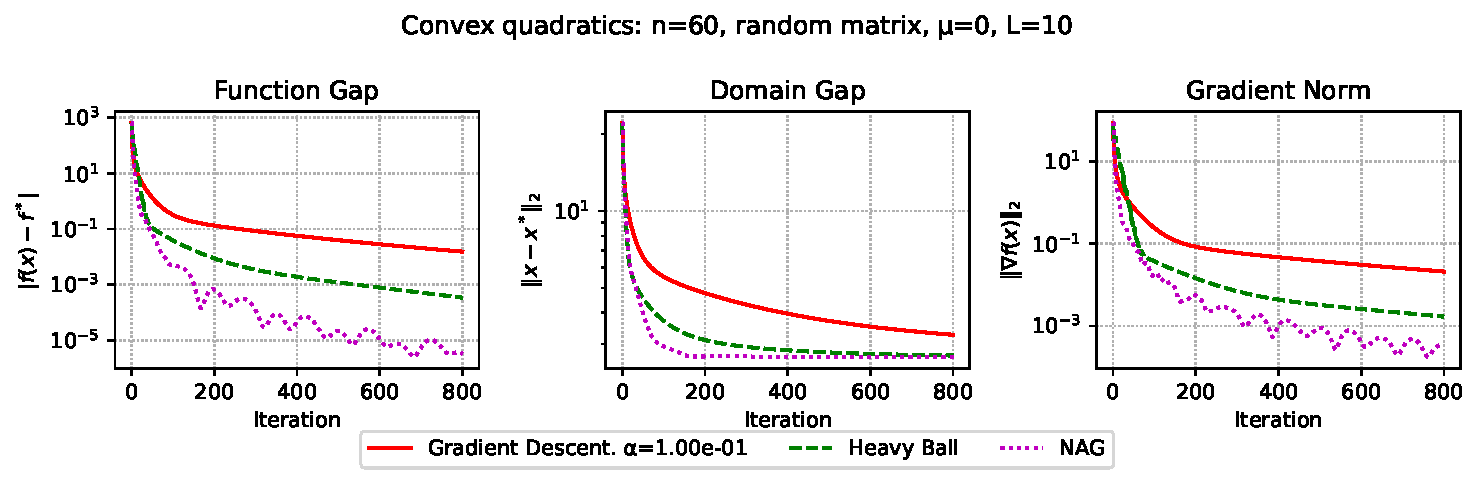
\includegraphics[keepaspectratio]{agd_random_0_10_60.pdf}}

\subsection{Сильно выпуклая квадратичная задача (регуляризованная
линейная
регрессия)}\label{ux441ux438ux43bux44cux43dux43e-ux432ux44bux43fux443ux43aux43bux430ux44f-ux43aux432ux430ux434ux440ux430ux442ux438ux447ux43dux430ux44f-ux437ux430ux434ux430ux447ux430-ux440ux435ux433ux443ux43bux44fux440ux438ux437ux43eux432ux430ux43dux43dux430ux44f-ux43bux438ux43dux435ux439ux43dux430ux44f-ux440ux435ux433ux440ux435ux441ux441ux438ux44f}

\pandocbounded{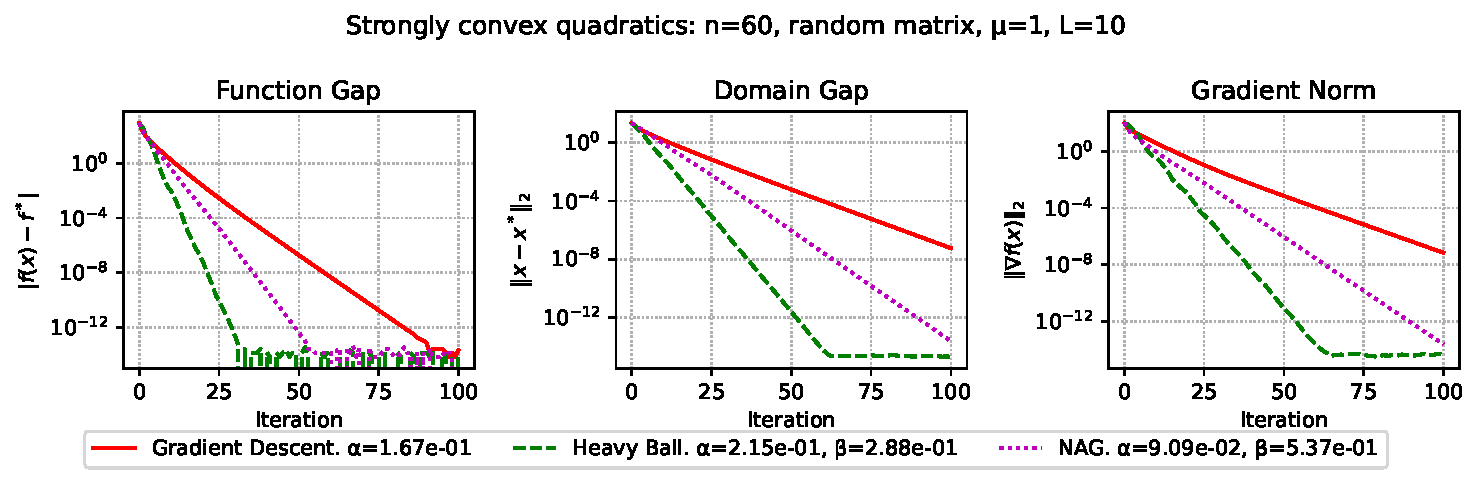
\includegraphics[keepaspectratio]{agd_random_1_10_60.pdf}}

\pandocbounded{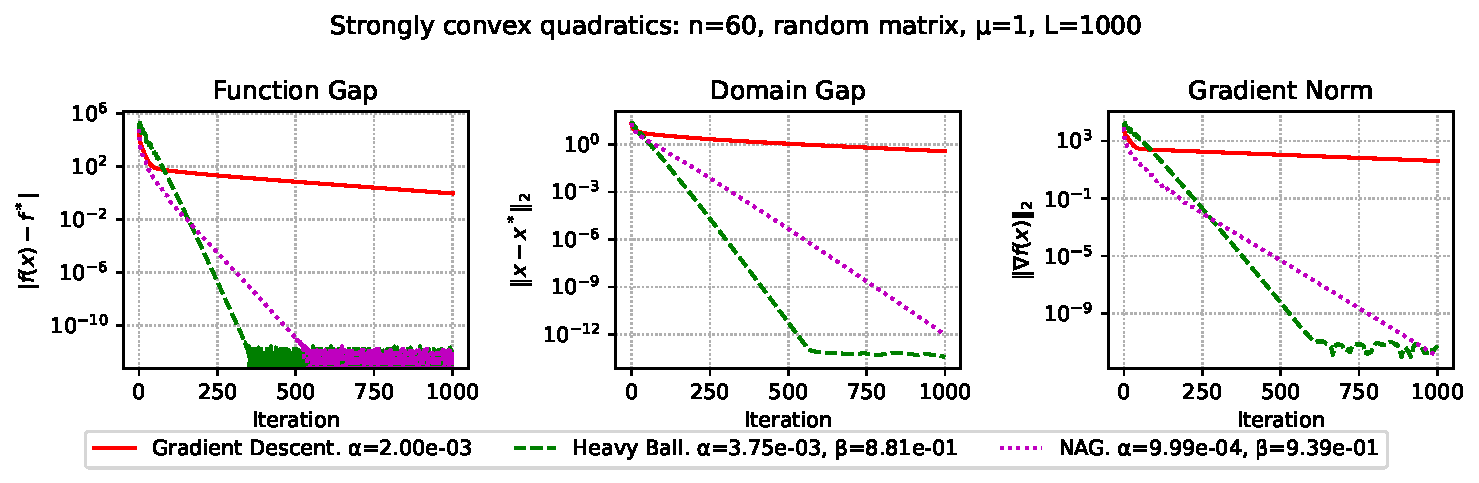
\includegraphics[keepaspectratio]{agd_random_1_1000_60.pdf}}

\pandocbounded{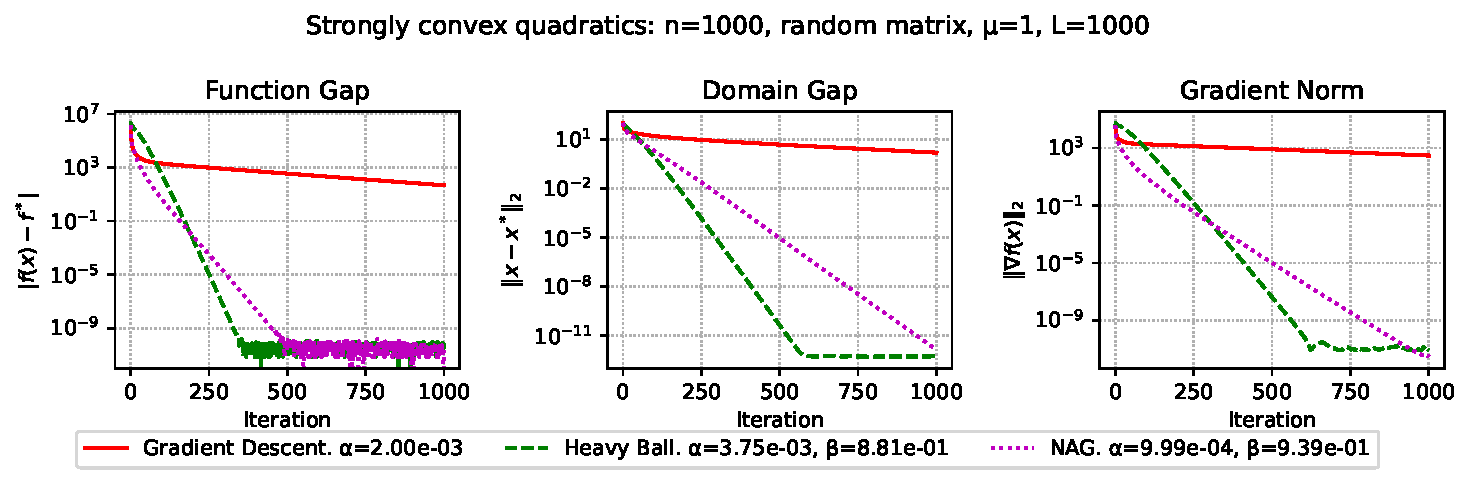
\includegraphics[keepaspectratio]{agd_random_1_1000_1000.pdf}}

\subsection{Выпуклая бинарная логистическая
регрессия}\label{ux432ux44bux43fux443ux43aux43bux430ux44f-ux431ux438ux43dux430ux440ux43dux430ux44f-ux43bux43eux433ux438ux441ux442ux438ux447ux435ux441ux43aux430ux44f-ux440ux435ux433ux440ux435ux441ux441ux438ux44f}

\pandocbounded{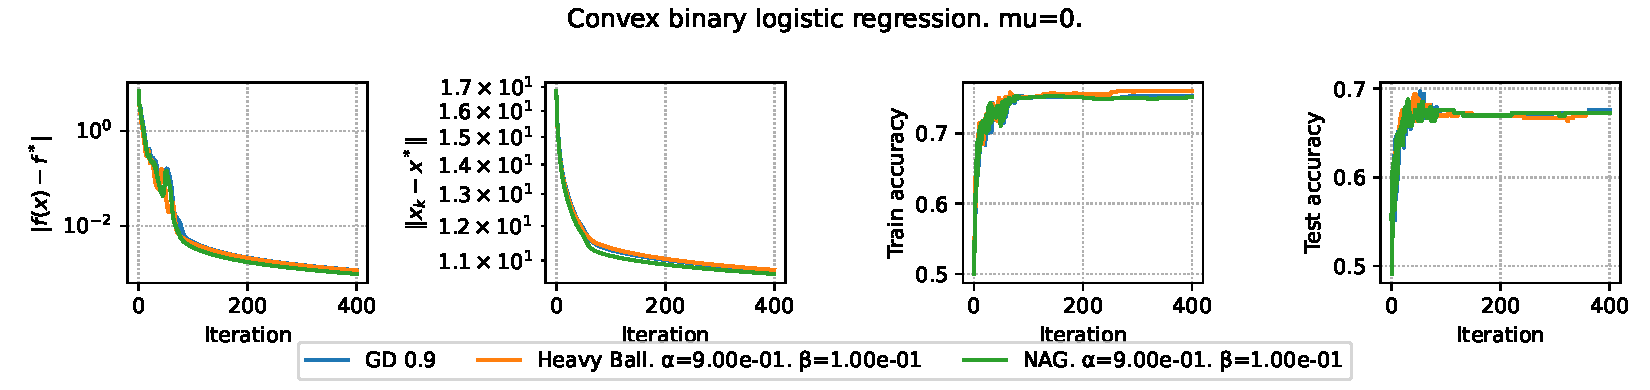
\includegraphics[keepaspectratio]{agd_convex_logreg_beta_0.1.pdf}}

\pandocbounded{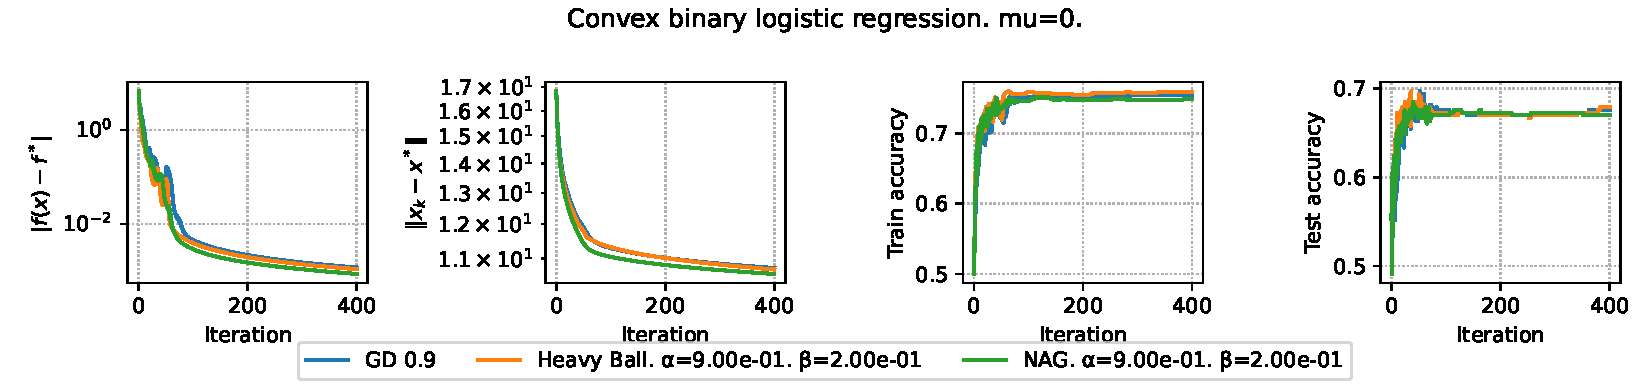
\includegraphics[keepaspectratio]{agd_convex_logreg_beta_0.2.pdf}}

\pandocbounded{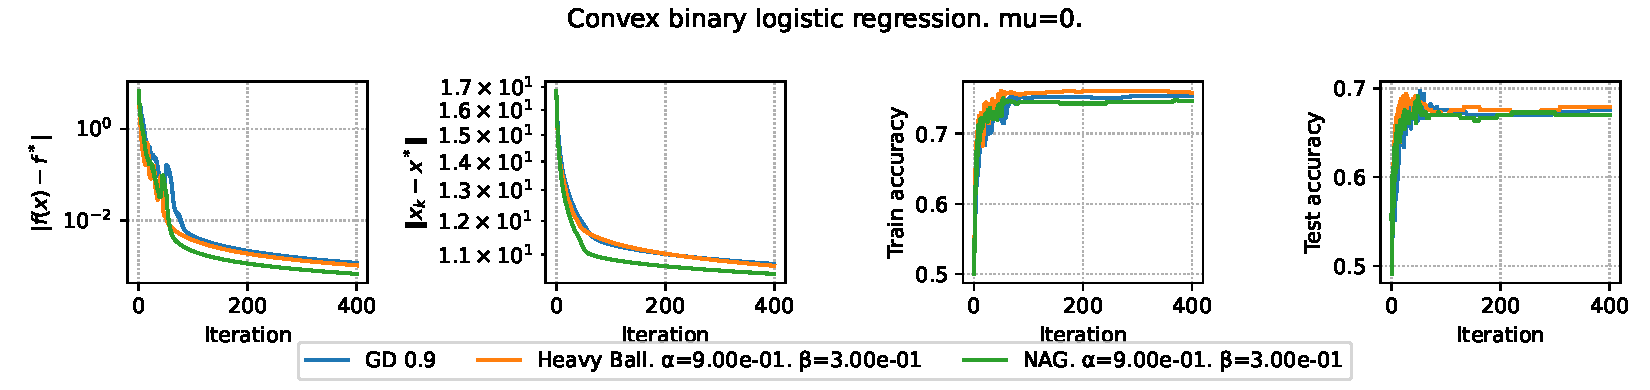
\includegraphics[keepaspectratio]{agd_convex_logreg_beta_0.3.pdf}}

\pandocbounded{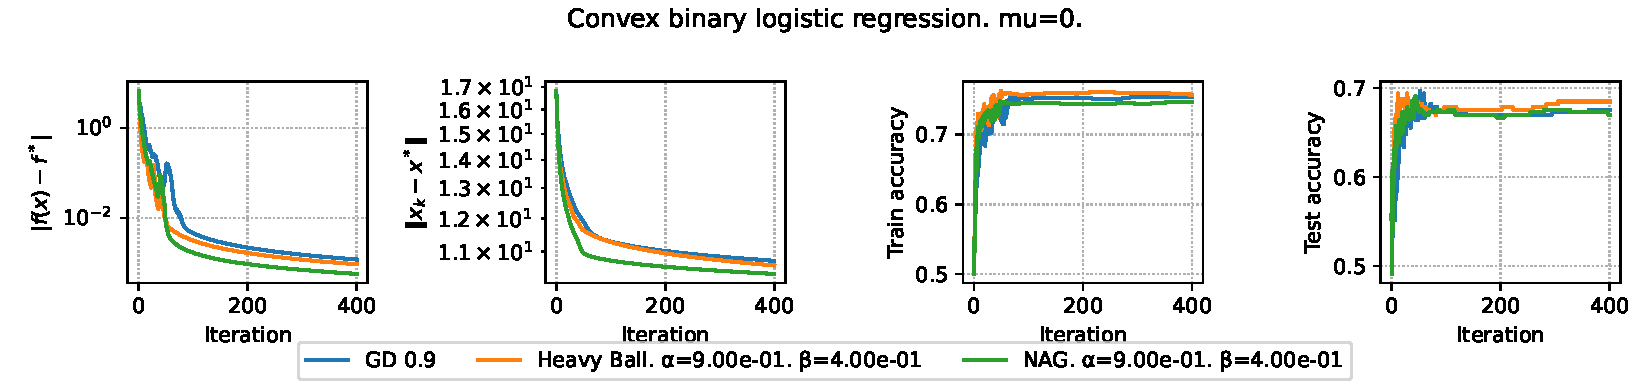
\includegraphics[keepaspectratio]{agd_convex_logreg_beta_0.4.pdf}}

\pandocbounded{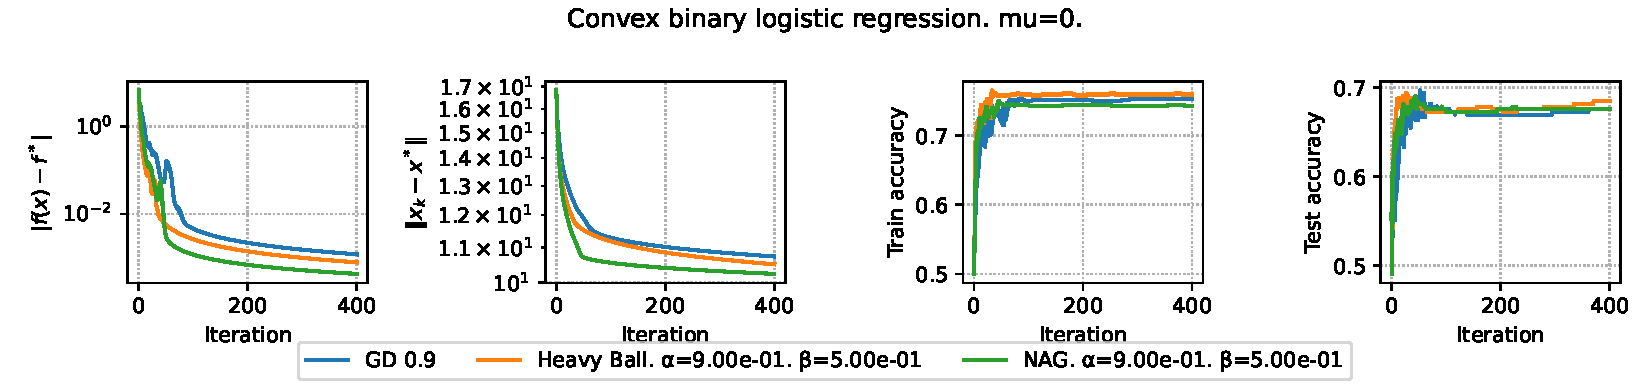
\includegraphics[keepaspectratio]{agd_convex_logreg_beta_0.5.pdf}}

\pandocbounded{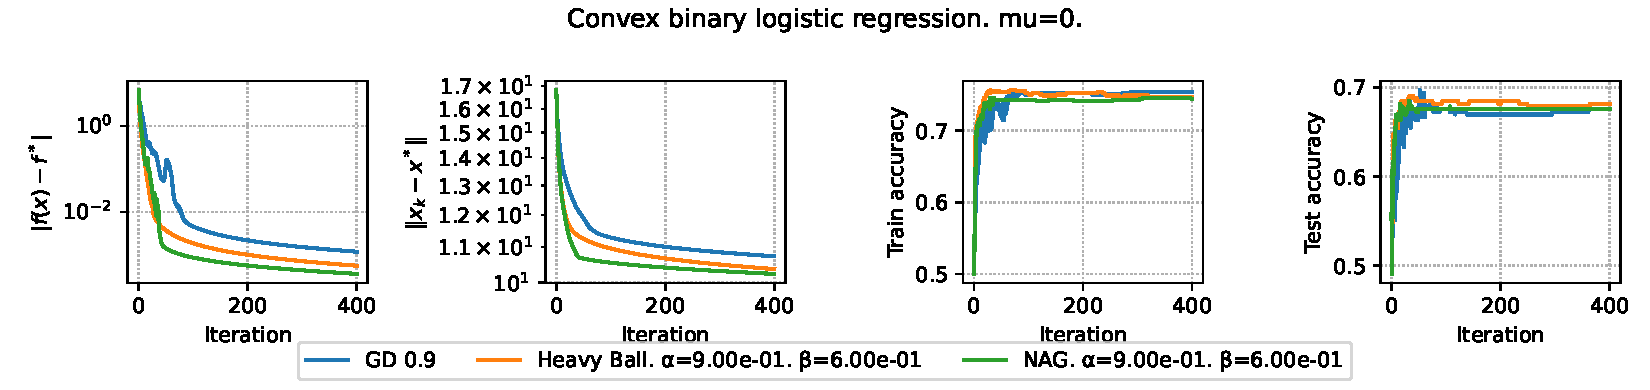
\includegraphics[keepaspectratio]{agd_convex_logreg_beta_0.6.pdf}}

\pandocbounded{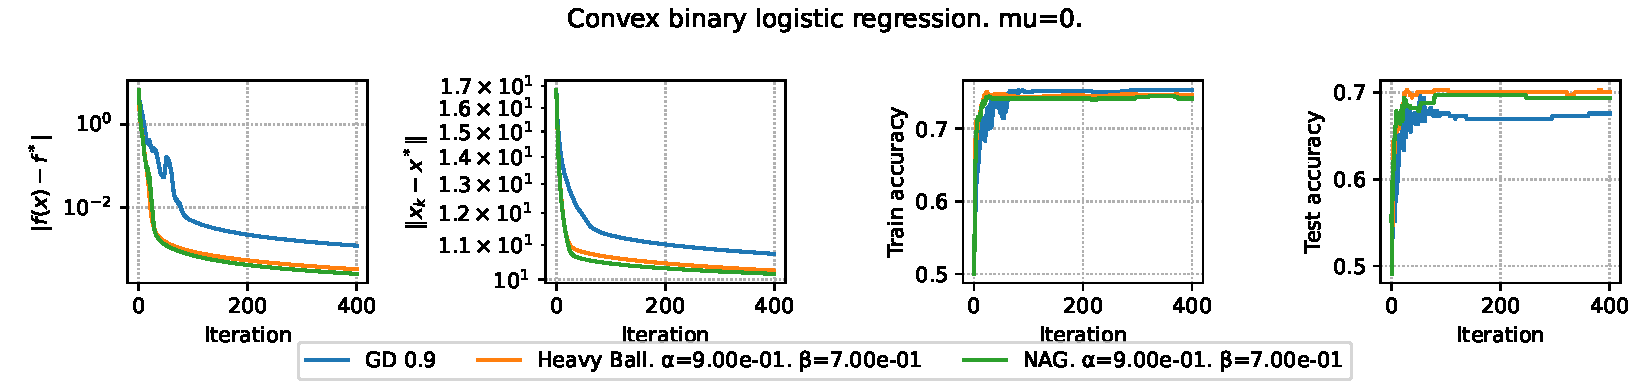
\includegraphics[keepaspectratio]{agd_convex_logreg_beta_0.7.pdf}}

\pandocbounded{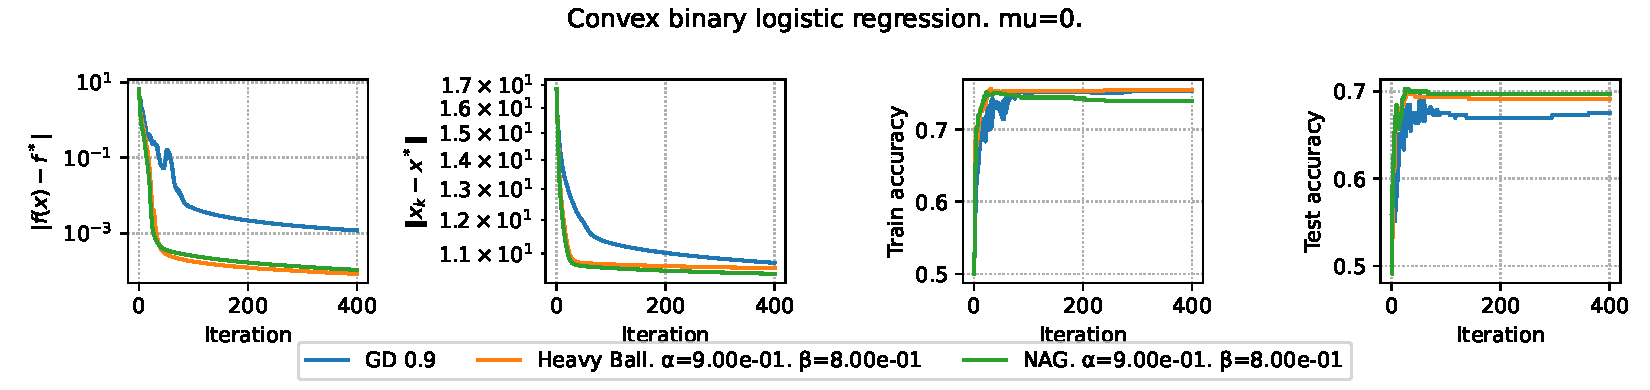
\includegraphics[keepaspectratio]{agd_convex_logreg_beta_0.8.pdf}}

\pandocbounded{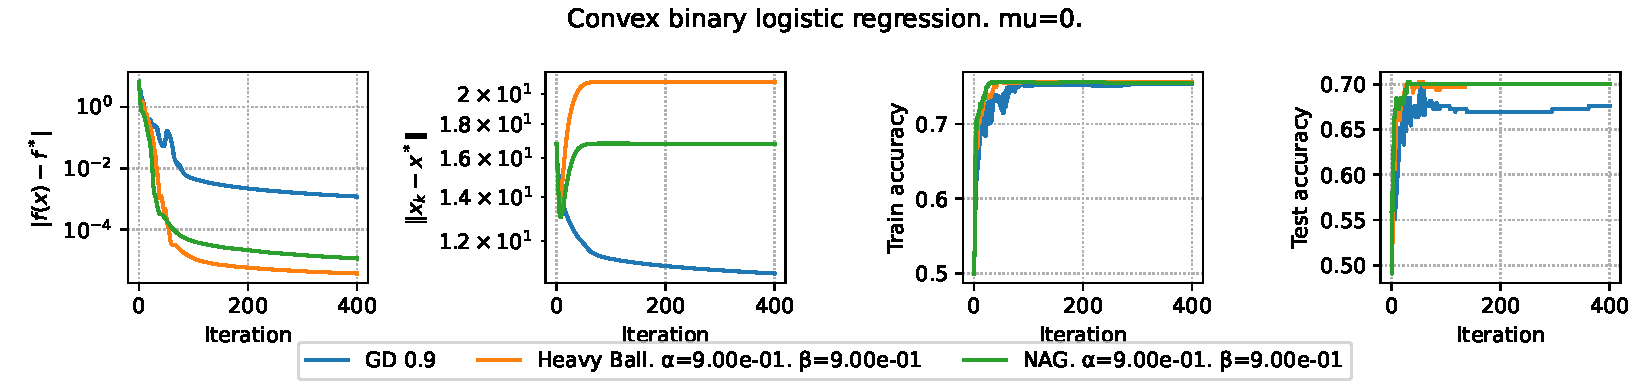
\includegraphics[keepaspectratio]{agd_convex_logreg_beta_0.9.pdf}}

\pandocbounded{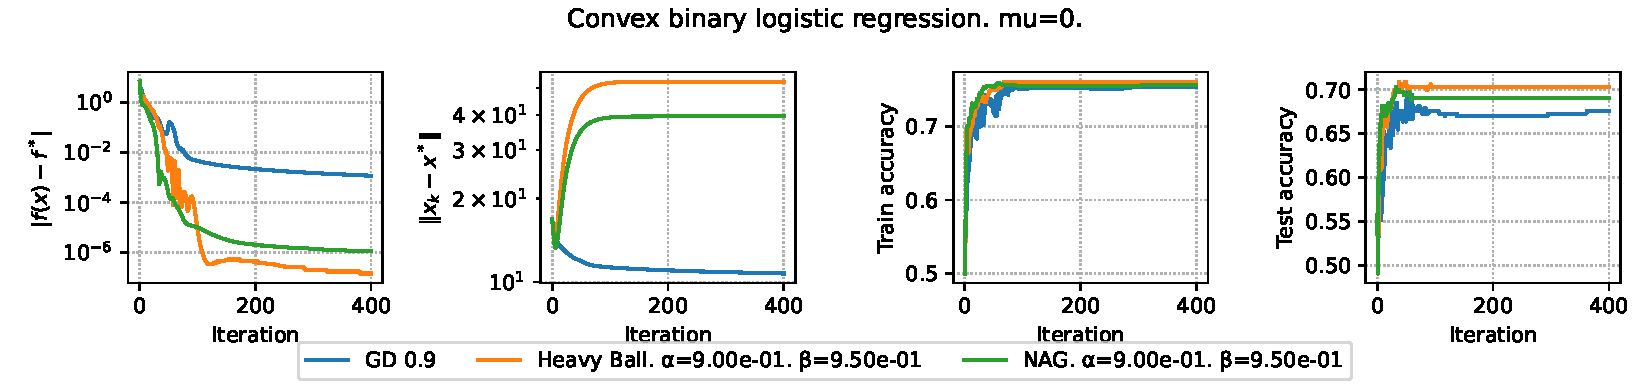
\includegraphics[keepaspectratio]{agd_convex_logreg_beta_0.95.pdf}}

\pandocbounded{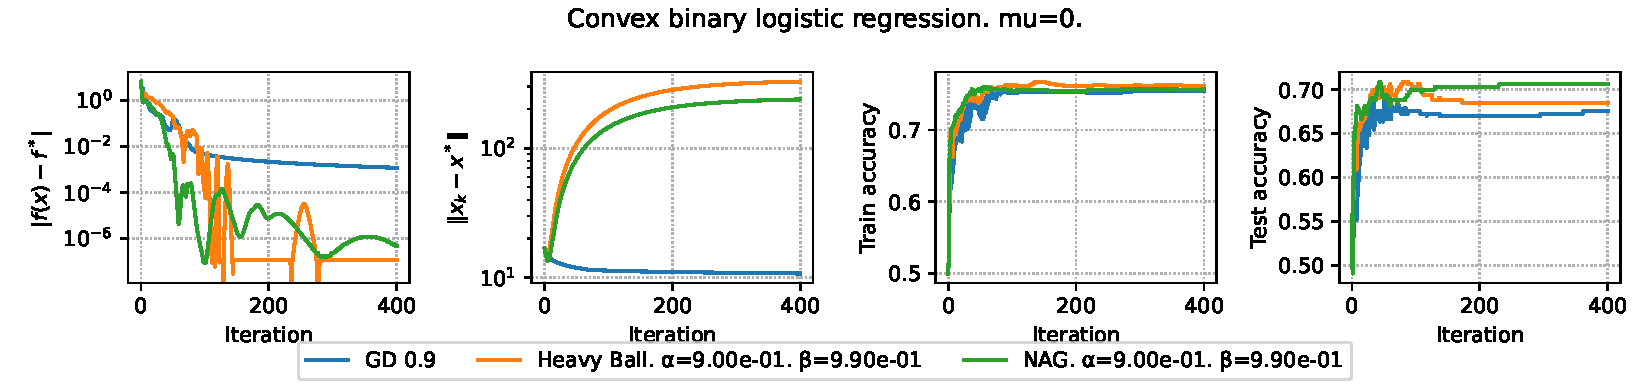
\includegraphics[keepaspectratio]{agd_convex_logreg_beta_0.99.pdf}}

\subsection{Сильно выпуклая бинарная логистическая
регрессия}\label{ux441ux438ux43bux44cux43dux43e-ux432ux44bux43fux443ux43aux43bux430ux44f-ux431ux438ux43dux430ux440ux43dux430ux44f-ux43bux43eux433ux438ux441ux442ux438ux447ux435ux441ux43aux430ux44f-ux440ux435ux433ux440ux435ux441ux441ux438ux44f}

\pandocbounded{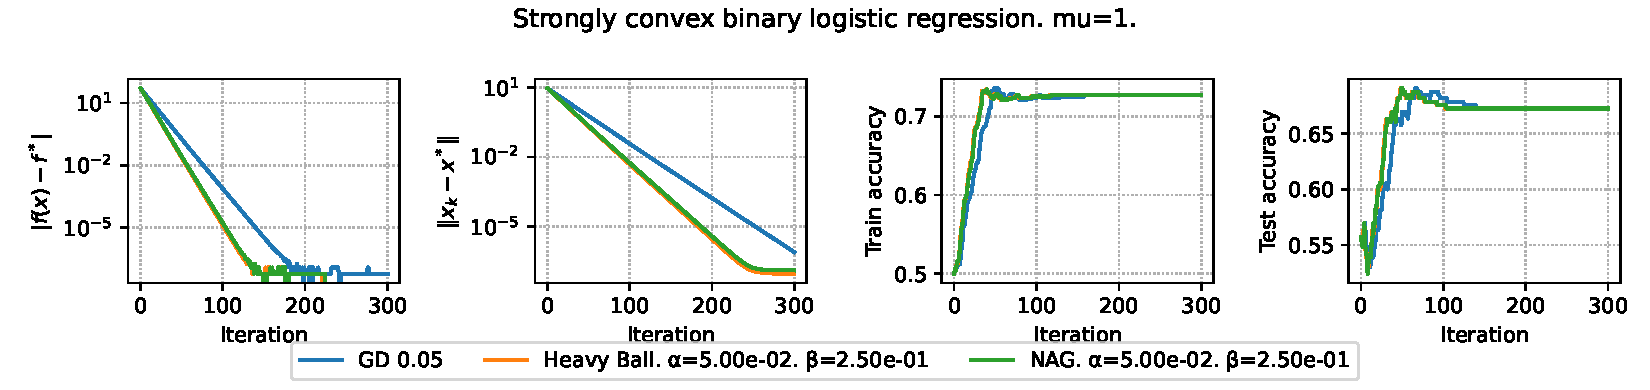
\includegraphics[keepaspectratio]{agd_strongly_convex_logreg_0.25.pdf}}

\pandocbounded{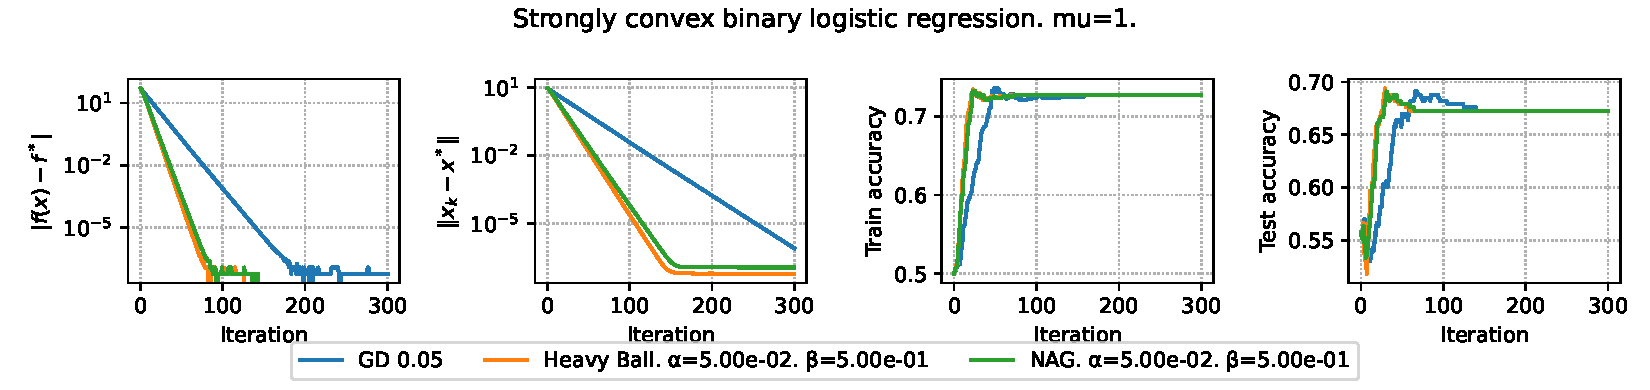
\includegraphics[keepaspectratio]{agd_strongly_convex_logreg_0.5.pdf}}

\pandocbounded{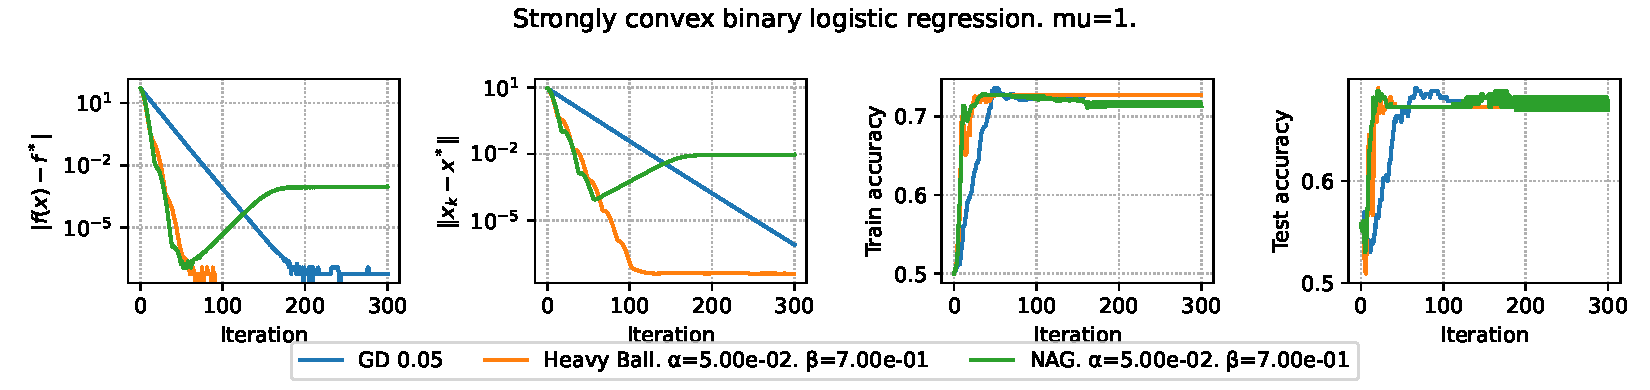
\includegraphics[keepaspectratio]{agd_strongly_convex_logreg_0.7.pdf}}

\pandocbounded{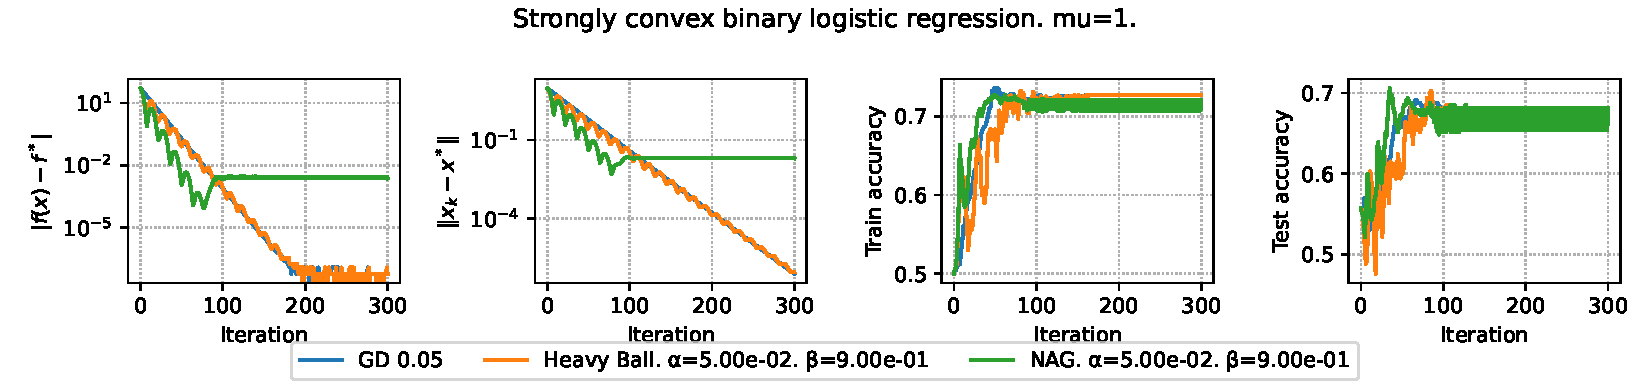
\includegraphics[keepaspectratio]{agd_strongly_convex_logreg_0.9.pdf}}

\subsection{\texorpdfstring{Нижние оценки для методов I порядка
\href{https://opt-eng-ana.github.io/blog/2025/opt-summary/}{(\faLink источник)}}{Нижние оценки для методов I порядка (источник)}}\label{ux43dux438ux436ux43dux438ux435-ux43eux446ux435ux43dux43aux438-ux434ux43bux44f-ux43cux435ux442ux43eux434ux43eux432-i-ux43fux43eux440ux44fux434ux43aux430-ux438ux441ux442ux43eux447ux43dux438ux43a}

\tiny

\begin{longtable}[]{@{}
  >{\raggedright\arraybackslash}p{(\linewidth - 10\tabcolsep) * \real{0.3038}}
  >{\centering\arraybackslash}p{(\linewidth - 10\tabcolsep) * \real{0.1646}}
  >{\centering\arraybackslash}p{(\linewidth - 10\tabcolsep) * \real{0.1456}}
  >{\centering\arraybackslash}p{(\linewidth - 10\tabcolsep) * \real{0.1329}}
  >{\raggedright\arraybackslash}p{(\linewidth - 10\tabcolsep) * \real{0.1203}}
  >{\raggedright\arraybackslash}p{(\linewidth - 10\tabcolsep) * \real{0.1329}}@{}}
\toprule\noalign{}
\begin{minipage}[b]{\linewidth}\raggedright
Тип задачи
\end{minipage} & \begin{minipage}[b]{\linewidth}\centering
Критерий
\end{minipage} & \begin{minipage}[b]{\linewidth}\centering
Нижняя оценка
\end{minipage} & \begin{minipage}[b]{\linewidth}\centering
Верхняя оценка
\end{minipage} & \begin{minipage}[b]{\linewidth}\raggedright
Ссылка (Ниж.)
\end{minipage} & \begin{minipage}[b]{\linewidth}\raggedright
Ссылка (Верх.)
\end{minipage} \\
\midrule\noalign{}
\endhead
\bottomrule\noalign{}
\endlastfoot
\(L\)-гладкая выпуклая & Зазор оптимальности &
\(\Omega\!\left(\sqrt{L\,\varepsilon^{-1}}\right)\) & \faCheck (точное
совпадение) & {[}1{]}, Теорема 2.1.7 & {[}1{]}, Теорема 2.2.2 \\
\(L\)-гладкая \(\mu\)-сильно выпуклая & Зазор оптимальности &
\(\Omega\!\left(\sqrt{\varkappa}\,\log \tfrac{1}{\varepsilon}\right)\) &
\faCheck & {[}1{]}, Теорема 2.1.13 & {[}1{]}, Теорема 2.2.2 \\
Негладкая \(G\)-липшицева выпуклая & Зазор оптимальности &
\(\Omega\!\left(G^{2}\,\varepsilon^{-2}\right)\) & \faCheck (точное
совпадение) & {[}1{]}, Теорема 3.2.1 & {[}1{]}, Теорема 3.2.2 \\
Негладкая \(G\)-липшицева \(\mu\)-сильно выпуклая & Зазор оптимальности
& \(\Omega\!\left(G^{2}\,(\mu\varepsilon)^{-1}\right)\) & \faCheck &
{[}1{]}, Теорема 3.2.5 & {[}3{]}, Теорема 3.9 \\
\(L\)-гладкая выпуклая (сходимость по функции) & Стационарность &
\(\Omega\!\left(\sqrt{\Delta L}\,\varepsilon^{-1}\right)\) & \faCheck (с
точностью до логарифмического множителя) & {[}2{]}, Теорема 1 & {[}2{]},
Приложение A.1 \\
\(L\)-гладкая выпуклая (сходимость по аргументу) & Стационарность &
\(\Omega\!\left(\sqrt{D L}\,\varepsilon^{-1/2}\right)\) & \faCheck &
{[}2{]}, Теорема 1 & {[}6{]}, Раздел 6.5 \\
\(L\)-гладкая невыпуклая & Стационарность &
\(\Omega\!\left(\Delta L\,\varepsilon^{-2}\right)\) & \faCheck &
{[}5{]}, Теорема 1 & {[}7{]}, Теорема 10.15 \\
Негладкая \(G\)-липшицева \(\rho\)-слабо выпуклая (WC) &
Квази-стационарность & Неизвестно &
\(\mathcal{O}\!\left(\varepsilon^{-4}\right)\) & / & {[}8{]}, Следствие
2.2 \\
\(L\)-гладкая \(\mu\)-PL & Зазор оптимальности &
\(\Omega\!\left(\varkappa \log \tfrac{1}{\varepsilon}\right)\) &
\faCheck & {[}9{]}, Теорема 3 & {[}10{]}, Теорема 1 \\
\end{longtable}

\normalsize

Источники:

\begin{itemize}
\tightlist
\item
  {[}1{]} - Lectures on Convex Optimization, Y. Nesterov.
\item
  {[}2{]} - Lower bounds for finding stationary points II: first-order
  methods, Y. Carmon, J.C. Duchi, O. Hinder, A. Sidford.
\item
  {[}3{]} - Convex optimization: Algorithms and complexity, S. Bubeck,
  others.
\item
  {[}4{]} - Optimizing the efficiency of first-order methods for
  decreasing the gradient of smooth convex functions D. Kim, J.A.
  Fessler.
\item
  {[}5{]} - Lower bounds for finding stationary points I, Y. Carmon,
  J.C. Duchi, O. Hinder, A. Sidford.
\item
  {[}6{]} - Optimizing the efficiency of first-order methods for
  decreasing the gradient of smooth convex functions, D. Kim, J.A.
  Fessler.
\item
  {[}7{]} - First-order methods in optimization, A. Beck. SIAM. 2017.
\item
  {[}8{]} - Stochastic subgradient method converges at the rate \$ O
  (k\^{}\{-1/4\}) \$ on weakly convex functions, D. Davis, D.
  Drusvyatskiy.
\item
  {[}9{]} - On the lower bound of minimizing Polyak-Lojasiewicz
  functions, P. Yue, C. Fang, Z. Lin.
\item
  {[}10{]} - Linear convergence of gradient and proximal-gradient
  methods under the Polyak-Lojasiewicz condition, H. Karimi, J. Nutini,
  M. Schmidt.
\end{itemize}

Обозначения:

\begin{itemize}
\tightlist
\item
  Зазор оптимальности: \(f(x_k) - f^* \leq \varepsilon\)
\item
  Стационарность: \(\|\nabla f(x_k)\| \leq \varepsilon\)
\item
  Квази-стационарность: \(\|\nabla f_\lambda(x_k)\| \leq \varepsilon\),
  где
  \(f_\lambda(x) = \inf\limits_{y \in \mathbb{R}^n} \left(f(y) + \frac{1}{2\lambda}\|y - x\|^2\right)\)
\item
  Липшицевость функции:
  \(|f(x) - f(y)| \leq G \|x - y\| \forall x, y \in \mathbb{R}^n\)
\item
  Липшицевость градиента (\(L\)-гладкость):
  \(\|\nabla f(x) - \nabla f(y)\| \leq L \|x - y\| \forall x, y \in \mathbb{R}^n\)
\item
  \(\mu\)-сильная выпуклость:
  \(f(\lambda x + (1 - \lambda)y) \le \lambda f(x) + (1 - \lambda)f(y) - \frac{\mu}{2} \lambda (1 - \lambda)\|x - y\|^2\)
\item
  \(\rho\)-слабо выпуклая функция:
  \(f(\lambda x + (1 - \lambda)y) \le \lambda f(x) + (1 - \lambda)f(y) + \rho \lambda (1 - \lambda)\|x - y\|^2 \forall x, y \in \mathbb{R}^n\)
\item
  Число обусловленности: \(\varkappa = \frac{L}{\mu}\)
\item
  Зазор в начальной точке: \(f(x_0) - f^* \leq \Delta\)
\item
  Зазор по аргументу: \(D = \|x_0 - x^*\|\)
\end{itemize}

\normalsize

\section{Задачи на
дом}\label{ux437ux430ux434ux430ux447ux438-ux43dux430-ux434ux43eux43c}

\begin{enumerate}
\def\labelenumi{\arabic{enumi}.}
\item
  \textbf{Локальная сходимость метода тяжелого шарика.} {[}20 баллов{]}
  Мы будем работать с методом тяжелого шарика

  \[
   \tag{HB}
   x_{k+1} = x_k - \alpha \nabla f(x_k) + \beta (x_k - x_{k-1})
   \]

  Известно, что для квадратичных функций оптимальный выбор
  гиперпараметров равен
  \(\alpha^* = \dfrac{4}{(\sqrt{L} + \sqrt{\mu})^2}, \beta^* = \dfrac{(\sqrt{L} - \sqrt{\mu})^2}{(\sqrt{L} + \sqrt{\mu})^2}\),
  который обеспечивает ускоренную линейную сходимость для сильно
  выпуклой квадратичной функции.

  Рассмотрим следующую непрерывно дифференцируемую, сильно выпуклую с
  параметром \(\mu\), и гладкую с параметром \(L\) функцию:

  \[
   f(x) = 
   \begin{cases} 
   \frac{25}{2}x^2, & \text{if } x < 1 \\
   \frac12x^2 + 24x - 12, & \text{if } 1 \leq x < 2 \\
   \frac{25}{2}x^2 - 24x + 36, & \text{if } x \geq 2
   \end{cases}
   \quad
   \nabla f(x) = 
   \begin{cases} 
   25x, & \text{if } x < 1 \\
   x + 24, & \text{if } 1 \leq x < 2 \\
   25x - 24, & \text{if } x \geq 2
   \end{cases}
   \]

  \begin{enumerate}
  \def\labelenumii{\arabic{enumii}.}
  \item
    Как доказать, что данная функция является выпуклой? Сильно выпуклой?
    Гладкой?
  \item
    Найдите константы \(\mu\) и \(L\) для данной функции.
  \item
    Постройте график функции для \(x \in [-4, 4]\).
  \item
    Запустите метод тяжелого шарика для функции с оптимальными
    гиперпараметрами
    \(\alpha^* = \dfrac{4}{(\sqrt{L} + \sqrt{\mu})^2}, \beta^* = \dfrac{(\sqrt{L} - \sqrt{\mu})^2}{(\sqrt{L} + \sqrt{\mu})^2}\)
    для квадратичной функции, начиная с \(x_0 = 3.5\). Если вы все
    сделали правильно, вы должны получить что-то вроде

    \href{https://drive.google.com/file/d/1HN_Hu4DKYoSvUrtbLbjEm79LRsiUlK8r/view?usp=sharing}{(heavy\_ball\_conv.mp4)}

    Вы можете использовать следующий код для построения:

\begin{Shaded}
\begin{Highlighting}[]
\ImportTok{import}\NormalTok{ numpy }\ImportTok{as}\NormalTok{ np}
\ImportTok{import}\NormalTok{ matplotlib.pyplot }\ImportTok{as}\NormalTok{ plt}
\ImportTok{import}\NormalTok{ matplotlib.animation }\ImportTok{as}\NormalTok{ animation}
\ImportTok{from}\NormalTok{ IPython.display }\ImportTok{import}\NormalTok{ HTML}

\CommentTok{\# Gradient of the function}
\KeywordTok{def}\NormalTok{ grad\_f(x):}
\NormalTok{    ...}

\CommentTok{\# Heavy Ball method implementation}
\KeywordTok{def}\NormalTok{ heavy\_ball\_method(alpha, beta, x0, num\_iterations):}
\NormalTok{    x }\OperatorTok{=}\NormalTok{ np.zeros(num\_iterations }\OperatorTok{+} \DecValTok{1}\NormalTok{)}
\NormalTok{    x\_prev }\OperatorTok{=}\NormalTok{ x0}
\NormalTok{    x\_curr }\OperatorTok{=}\NormalTok{ x0  }\CommentTok{\# Initialize x[1] same as x[0] to start the algorithm}
    \ControlFlowTok{for}\NormalTok{ i }\KeywordTok{in} \BuiltInTok{range}\NormalTok{(num\_iterations):}
\NormalTok{        x[i] }\OperatorTok{=}\NormalTok{ x\_curr}
\NormalTok{        x\_new }\OperatorTok{=}\NormalTok{ x\_curr }\OperatorTok{{-}}\NormalTok{ alpha }\OperatorTok{*}\NormalTok{ grad\_f(x\_curr) }\OperatorTok{+}\NormalTok{ beta }\OperatorTok{*}\NormalTok{ (x\_curr }\OperatorTok{{-}}\NormalTok{ x\_prev)}
\NormalTok{        x\_prev }\OperatorTok{=}\NormalTok{ x\_curr}
\NormalTok{        x\_curr }\OperatorTok{=}\NormalTok{ x\_new}
\NormalTok{    x[num\_iterations] }\OperatorTok{=}\NormalTok{ x\_curr}
    \ControlFlowTok{return}\NormalTok{ x}

\CommentTok{\# Parameters}
\NormalTok{L }\OperatorTok{=}\NormalTok{ ...}
\NormalTok{mu }\OperatorTok{=}\NormalTok{ ...}
\NormalTok{alpha\_star }\OperatorTok{=}\NormalTok{ ...}
\NormalTok{beta\_star }\OperatorTok{=}\NormalTok{ ...}
\NormalTok{x0 }\OperatorTok{=}\NormalTok{ ...}
\NormalTok{num\_iterations }\OperatorTok{=} \DecValTok{30}

\CommentTok{\# Generate the trajectory of the method}
\NormalTok{trajectory }\OperatorTok{=}\NormalTok{ heavy\_ball\_method(alpha\_star, beta\_star, x0, num\_iterations)}

\CommentTok{\# Setup the figure and axes for the animation}
\NormalTok{fig, (ax1, ax2) }\OperatorTok{=}\NormalTok{ plt.subplots(}\DecValTok{1}\NormalTok{, }\DecValTok{2}\NormalTok{, figsize}\OperatorTok{=}\NormalTok{(}\DecValTok{7}\NormalTok{, }\FloatTok{3.5}\NormalTok{))}
\NormalTok{fig.suptitle(}\StringTok{"Heavy ball method with optimal hyperparameters α* β*"}\NormalTok{)}

\CommentTok{\# Function for updating the animation}
\KeywordTok{def}\NormalTok{ update(i):}
\NormalTok{    ax1.clear()}
\NormalTok{    ax2.clear()}

    \CommentTok{\# Plot f(x) and trajectory}
\NormalTok{    x\_vals }\OperatorTok{=}\NormalTok{ np.linspace(}\OperatorTok{{-}}\DecValTok{4}\NormalTok{, }\DecValTok{4}\NormalTok{, }\DecValTok{100}\NormalTok{)}
\NormalTok{    f\_vals }\OperatorTok{=}\NormalTok{ np.piecewise(x\_vals, [x\_vals }\OperatorTok{\textless{}} \DecValTok{1}\NormalTok{, (x\_vals }\OperatorTok{\textgreater{}=} \DecValTok{1}\NormalTok{) }\OperatorTok{\&}\NormalTok{ (x\_vals }\OperatorTok{\textless{}} \DecValTok{2}\NormalTok{), x\_vals }\OperatorTok{\textgreater{}=} \DecValTok{2}\NormalTok{],}
\NormalTok{                        [}\KeywordTok{lambda}\NormalTok{ x: }\FloatTok{12.5} \OperatorTok{*}\NormalTok{ x}\OperatorTok{**}\DecValTok{2}\NormalTok{, }\KeywordTok{lambda}\NormalTok{ x: }\FloatTok{.5} \OperatorTok{*}\NormalTok{ x}\OperatorTok{**}\DecValTok{2} \OperatorTok{+} \DecValTok{24} \OperatorTok{*}\NormalTok{ x }\OperatorTok{{-}} \DecValTok{12}\NormalTok{, }\KeywordTok{lambda}\NormalTok{ x: }\FloatTok{12.5} \OperatorTok{*}\NormalTok{ x}\OperatorTok{**}\DecValTok{2} \OperatorTok{{-}} \DecValTok{24} \OperatorTok{*}\NormalTok{ x }\OperatorTok{+} \DecValTok{36}\NormalTok{])}
\NormalTok{    ax1.plot(x\_vals, f\_vals, }\StringTok{\textquotesingle{}b{-}\textquotesingle{}}\NormalTok{)}
\NormalTok{    ax1.plot(trajectory[:i], [}\FloatTok{12.5} \OperatorTok{*}\NormalTok{ x}\OperatorTok{**}\DecValTok{2} \ControlFlowTok{if}\NormalTok{ x }\OperatorTok{\textless{}} \DecValTok{1} \ControlFlowTok{else} \FloatTok{.5} \OperatorTok{*}\NormalTok{ x}\OperatorTok{**}\DecValTok{2} \OperatorTok{+} \DecValTok{24} \OperatorTok{*}\NormalTok{ x }\OperatorTok{{-}} \DecValTok{12} \ControlFlowTok{if}\NormalTok{ x }\OperatorTok{\textless{}} \DecValTok{2} \ControlFlowTok{else} \FloatTok{12.5} \OperatorTok{*}\NormalTok{ x}\OperatorTok{**}\DecValTok{2} \OperatorTok{{-}} \DecValTok{24} \OperatorTok{*}\NormalTok{ x }\OperatorTok{+} \DecValTok{36} \ControlFlowTok{for}\NormalTok{ x }\KeywordTok{in}\NormalTok{ trajectory[:i]], }\StringTok{\textquotesingle{}ro{-}\textquotesingle{}}\NormalTok{)}
    \CommentTok{\# Add vertical dashed lines at x=1 and x=2 on the left subplot}
\NormalTok{    ax1.axvline(x}\OperatorTok{=}\DecValTok{1}\NormalTok{, color}\OperatorTok{=}\StringTok{\textquotesingle{}navy\textquotesingle{}}\NormalTok{, linestyle}\OperatorTok{=}\StringTok{\textquotesingle{}{-}{-}\textquotesingle{}}\NormalTok{)}
\NormalTok{    ax1.axvline(x}\OperatorTok{=}\DecValTok{2}\NormalTok{, color}\OperatorTok{=}\StringTok{\textquotesingle{}navy\textquotesingle{}}\NormalTok{, linestyle}\OperatorTok{=}\StringTok{\textquotesingle{}{-}{-}\textquotesingle{}}\NormalTok{)}

    \CommentTok{\# Plot function value from iteration}
\NormalTok{    f\_trajectory }\OperatorTok{=}\NormalTok{ [}\VariableTok{None} \ControlFlowTok{for}\NormalTok{ x }\KeywordTok{in}\NormalTok{ trajectory]}
\NormalTok{    f\_trajectory[:i] }\OperatorTok{=}\NormalTok{ [}\FloatTok{12.5} \OperatorTok{*}\NormalTok{ x}\OperatorTok{**}\DecValTok{2} \ControlFlowTok{if}\NormalTok{ x }\OperatorTok{\textless{}} \DecValTok{1} \ControlFlowTok{else} \FloatTok{.5} \OperatorTok{*}\NormalTok{ x}\OperatorTok{**}\DecValTok{2} \OperatorTok{+} \DecValTok{24} \OperatorTok{*}\NormalTok{ x }\OperatorTok{{-}} \DecValTok{12} \ControlFlowTok{if}\NormalTok{ x }\OperatorTok{\textless{}} \DecValTok{2} \ControlFlowTok{else} \FloatTok{12.5} \OperatorTok{*}\NormalTok{ x}\OperatorTok{**}\DecValTok{2} \OperatorTok{{-}} \DecValTok{24} \OperatorTok{*}\NormalTok{ x }\OperatorTok{+} \DecValTok{36} \ControlFlowTok{for}\NormalTok{ x }\KeywordTok{in}\NormalTok{ trajectory[:i]]}
\NormalTok{    ax2.plot(}\BuiltInTok{range}\NormalTok{(}\BuiltInTok{len}\NormalTok{(trajectory)), f\_trajectory, }\StringTok{\textquotesingle{}ro{-}\textquotesingle{}}\NormalTok{)}
\NormalTok{    ax2.set\_xlim(}\DecValTok{0}\NormalTok{, }\BuiltInTok{len}\NormalTok{(trajectory))}
\NormalTok{    ax2.set\_ylim(}\BuiltInTok{min}\NormalTok{(f\_vals), }\BuiltInTok{max}\NormalTok{(f\_vals))}
    \CommentTok{\# Add horizontal dashed lines at f(1) and f(2) on the right subplot}
\NormalTok{    f\_1 }\OperatorTok{=} \FloatTok{12.5} \OperatorTok{*} \FloatTok{1.0}\OperatorTok{**}\DecValTok{2}
\NormalTok{    f\_2 }\OperatorTok{=} \FloatTok{.5} \OperatorTok{*} \FloatTok{2.}\OperatorTok{**}\DecValTok{2} \OperatorTok{+} \DecValTok{24} \OperatorTok{*} \FloatTok{2.} \OperatorTok{{-}} \DecValTok{12}
\NormalTok{    ax2.axhline(y}\OperatorTok{=}\NormalTok{f\_1, color}\OperatorTok{=}\StringTok{\textquotesingle{}navy\textquotesingle{}}\NormalTok{, linestyle}\OperatorTok{=}\StringTok{\textquotesingle{}{-}{-}\textquotesingle{}}\NormalTok{)}
\NormalTok{    ax2.axhline(y}\OperatorTok{=}\NormalTok{f\_2, color}\OperatorTok{=}\StringTok{\textquotesingle{}navy\textquotesingle{}}\NormalTok{, linestyle}\OperatorTok{=}\StringTok{\textquotesingle{}{-}{-}\textquotesingle{}}\NormalTok{)}

    \CommentTok{\# ax1.set\_title("Function f(x) and Trajectory")}
\NormalTok{    ax1.set\_xlabel(}\StringTok{"x"}\NormalTok{)}
\NormalTok{    ax1.set\_ylabel(}\StringTok{"f(x)"}\NormalTok{)}
\NormalTok{    ax1.grid(linestyle}\OperatorTok{=}\StringTok{":"}\NormalTok{)}

    \CommentTok{\# ax2.set\_title("Function Value from Iteration")}
\NormalTok{    ax2.set\_xlabel(}\StringTok{"Iteration"}\NormalTok{)}
\NormalTok{    ax2.set\_ylabel(}\StringTok{"f(x)"}\NormalTok{)}
\NormalTok{    ax2.grid(linestyle}\OperatorTok{=}\StringTok{":"}\NormalTok{)}

\NormalTok{    plt.tight\_layout()}

\CommentTok{\# Create the animation}
\NormalTok{ani }\OperatorTok{=}\NormalTok{ animation.FuncAnimation(fig, update, frames}\OperatorTok{=}\NormalTok{num\_iterations, repeat}\OperatorTok{=}\VariableTok{False}\NormalTok{, interval}\OperatorTok{=}\DecValTok{100}\NormalTok{)}
\NormalTok{HTML(ani.to\_jshtml())}
\end{Highlighting}
\end{Shaded}
  \item
    Измените начальную точку на \(x_0 = 3.4\). Что вы видите? Как можно
    назвать такое поведение метода?
  \item
    Измените гиперпараметры
    \(\alpha^{\text{Global}} = \frac2L, \beta^{\text{Global}} = \frac{\mu}{L}\)
    и запустите метод снова с \(x_0 = 3.4\). Проверьте, что вы получили
    ускоренную сходимость.
  \end{enumerate}

  Контекст: этот контрпример был предоставлен в
  \href{https://arxiv.org/pdf/1408.3595.pdf}{статье}, в то время как
  глобальная сходимость метода тяжелого шарика для общей гладкой сильно
  выпуклой функции была введена в другой
  \href{https://arxiv.org/pdf/1412.7457.pdf}{статье}. Недавно было
  \href{https://arxiv.org/pdf/2307.11291.pdf}{предложено}, что метод
  тяжелого шарика (HB) доказуемо не достигает ускоренной сходимости на
  гладких сильно выпуклых задачах.
\item
  {[}40 points{]} В этой задаче мы будем работать с ускоренными
  методами, применяемыми к задаче логистической регрессии. Хорошее
  визуальное введение по теме доступно
  \href{https://mlu-explain.github.io/logistic-regression/}{здесь}.

  Логистическая регрессия является стандартной моделью в задачах
  классификации. Для простоты рассмотрим только случай бинарной
  классификации. Интуитивно, задача формулируется следующим образом:
  Есть обучающая выборка \(\{(a_i, b_i)\}_{i=1}^m\), состоящая из \(m\)
  векторов \(a_i \in \mathbb{R}^n\) (относящихся к признакам) и
  соответствующих чисел \(b_i \in \{-1, 1\}\) (относящихся к классам или
  меткам). Цель состоит в том, чтобы построить алгоритм \(b(\cdot)\),
  который для любого нового вектора признаков \(a\) автоматически
  определяет его класс \(b(a) \in \{-1, 1\}\).

  В модели логистической регрессии класс определяется на основе знака
  линейной комбинации компонентов вектора \(a\) с некоторыми
  фиксированными коэффициентами \(x \in \mathbb{R}^n\):

  \[
   b(a) := \text{sign}(\langle a, x \rangle).
   \]

  Коэффициенты \(x\) являются параметрами модели и подбираются путем
  решения следующей оптимизационной задачи:

  \[
   \tag{LogReg}
   \min_{x \in \mathbb{R}^n} \left( \frac{1}{m} \sum_{i=1}^m \ln(1 + \exp(-b_i \langle a_i, x \rangle)) + \frac{\lambda}{2} \|x\|^2 \right),
   \]

  где \(\lambda \geq 0\) является коэффициентом регуляризации
  (параметром модели).

  \begin{enumerate}
  \def\labelenumii{\arabic{enumii}.}
  \item
    Будет ли задача LogReg выпуклой для \(\lambda = 0\)? Каков градиент
    целевой функции? Будет ли она сильно выпуклой? Что будет, если вы
    добавите регуляризацию с \(\lambda > 0\)?
  \item
    Мы будем работать с реальными данными для \(A\) и \(b\): возьмите
    датасет mushrooms. Будьте осторожны, вам нужно будет предсказать,
    является ли гриб ядовитым или съедобным. Плохая модель может
    привести к смерти в этом упражнении.

\begin{Shaded}
\begin{Highlighting}[]
\ImportTok{import}\NormalTok{ requests}
\ImportTok{from}\NormalTok{ sklearn.datasets }\ImportTok{import}\NormalTok{ load\_svmlight\_file}

\CommentTok{\# URL of the file to download}
\NormalTok{url }\OperatorTok{=} \StringTok{\textquotesingle{}https://cu25.fmin.xyz/files/mushrooms.txt\textquotesingle{}}

\CommentTok{\# Download the file and save it locally}
\NormalTok{response }\OperatorTok{=}\NormalTok{ requests.get(url)}
\NormalTok{dataset }\OperatorTok{=} \StringTok{\textquotesingle{}mushrooms.txt\textquotesingle{}}

\CommentTok{\# Ensure the request was successful}
\ControlFlowTok{if}\NormalTok{ response.status\_code }\OperatorTok{==} \DecValTok{200}\NormalTok{:}
    \ControlFlowTok{with} \BuiltInTok{open}\NormalTok{(dataset, }\StringTok{\textquotesingle{}wb\textquotesingle{}}\NormalTok{) }\ImportTok{as}\NormalTok{ f:}
\NormalTok{        f.write(response.content)}

    \CommentTok{\# Load the dataset from the downloaded file}
\NormalTok{    data }\OperatorTok{=}\NormalTok{ load\_svmlight\_file(dataset)}
\NormalTok{    A, b }\OperatorTok{=}\NormalTok{ data[}\DecValTok{0}\NormalTok{].toarray(), data[}\DecValTok{1}\NormalTok{]}
\NormalTok{    n, d }\OperatorTok{=}\NormalTok{ A.shape}

    \BuiltInTok{print}\NormalTok{(}\StringTok{"Data loaded successfully."}\NormalTok{)}
    \BuiltInTok{print}\NormalTok{(}\SpecialStringTok{f"Number of samples: }\SpecialCharTok{\{}\NormalTok{n}\SpecialCharTok{\}}\SpecialStringTok{, Number of features: }\SpecialCharTok{\{}\NormalTok{d}\SpecialCharTok{\}}\SpecialStringTok{"}\NormalTok{)}
\ControlFlowTok{else}\NormalTok{:}
    \BuiltInTok{print}\NormalTok{(}\SpecialStringTok{f"Failed to download the file. Status code: }\SpecialCharTok{\{}\NormalTok{response}\SpecialCharTok{.}\NormalTok{status\_code}\SpecialCharTok{\}}\SpecialStringTok{"}\NormalTok{)}
\end{Highlighting}
\end{Shaded}
  \item
    Разделите данные на две части: обучение и тест. Мы будем обучать
    модель на \(A_{train}\), \(b_{train}\) и измерять точность модели на
    \(A_{test}\), \(b_{test}\).

\begin{Shaded}
\begin{Highlighting}[]
\ImportTok{from}\NormalTok{ sklearn.model\_selection }\ImportTok{import}\NormalTok{ train\_test\_split}
\CommentTok{\# Split the data into training and test sets}
\NormalTok{A\_train, A\_test, b\_train, b\_test }\OperatorTok{=}\NormalTok{ train\_test\_split(A, b, test\_size}\OperatorTok{=}\FloatTok{0.2}\NormalTok{, random\_state}\OperatorTok{=}\DecValTok{214}\NormalTok{)}
\end{Highlighting}
\end{Shaded}
  \item
    Для обучения \(A_{train}\), \(b_{train}\), оцените константы
    \(\mu, L\) задачи оптимизации. Используйте одно и то же маленькое
    значение \(\lambda\) для всех экспериментов
  \item
    Используя градиентный спуск с шагом \(\frac{1}{L}\), обучите модель.
    Постройте график: точность в зависимости от номера итерации.

    \[
     \tag{HB}
     x_{k+1} = x_k - \alpha \nabla f(x_k) + \beta (x_k - x_{k-1})
     \]

    Зафиксируйте шаг \(\alpha = \frac{1}{L}\) и найдите различные
    значения импульса \(\beta\) от \(-1\) до \(1\). Выберите свой
    собственный критерий сходимости и постройте сходимость для
    нескольких значений импульса на одном графике. Сходится ли она
    всегда монотонно?
  \item
    Для лучшего значения импульса \(\beta\), постройте зависимость
    точности модели на тестовой выборке от времени работы метода.
    Добавьте на тот же график сходимость градиентного спуска с шагом
    \(\frac{1}{L}\). Сделайте вывод. Убедитесь, что вы используете одно
    и то же значение \(\lambda\) для обоих методов.
  \item
    Решите задачу логистической регрессии с использованием метода
    Нэстерова.

    \[
     \tag{NAG}
     x_{k+1} = x_k - \alpha \nabla f(x_k + \beta (x_k - x_{k-1})) + \beta (x_k - x_{k-1})  
     \]

    Зафиксируйте шаг \(\frac{1}{L}\) и найдите различные значения
    импульса \(\beta\) от \(-1\) до \(1\). Проверьте также значения
    импульса равные \(\frac{k}{k+3}\), \(\frac{k}{k+2}\),
    \(\frac{k}{k+1}\) (\(k\) - число итераций), и если вы решаете сильно
    выпуклую задачу, также
    \(\frac{\sqrt{L} - \sqrt{\mu}}{\sqrt{L} + \sqrt{\mu}}\). Постройте
    сходимость метода в зависимости от числа итераций (выберите свой
    собственный критерий сходимости) для различных значений импульса.
    Сходится ли она всегда монотонно?
  \item
    Для лучшего значения импульса \(\beta\), постройте зависимость
    точности модели на тестовой выборке от времени работы метода.
    Добавьте этот график к графикам для тяжелого шарика и градиентного
    спуска из предыдущих шагов. Сделайте вывод.
  \item
    Теперь мы отбросим оценку значения \(L\) и будем пытаться сделать
    его адаптивным. Давайте сделаем выбор константы \(L\) адаптивным.

    \[
     f(y) \leq f(x^k) + \langle \nabla f(x^k), y - x^k \rangle + \frac{L}{2}\|x^k - y\|_2^2
     \]

    В частности, процедура может работать так:

\begin{Shaded}
\begin{Highlighting}[]
\KeywordTok{def}\NormalTok{ backtracking\_L(f, grad, x, h, L0, rho, maxiter}\OperatorTok{=}\DecValTok{100}\NormalTok{):}
\NormalTok{    L }\OperatorTok{=}\NormalTok{ L0}
\NormalTok{    fx }\OperatorTok{=}\NormalTok{ f(x)}
\NormalTok{    gradx }\OperatorTok{=}\NormalTok{ grad(x)}
    \BuiltInTok{iter} \OperatorTok{=} \DecValTok{0}
    \ControlFlowTok{while} \BuiltInTok{iter} \OperatorTok{\textless{}}\NormalTok{ maxiter :}
\NormalTok{        y }\OperatorTok{=}\NormalTok{ x }\OperatorTok{{-}} \DecValTok{1} \OperatorTok{/}\NormalTok{ L }\OperatorTok{*}\NormalTok{ h}
        \ControlFlowTok{if}\NormalTok{ f(y) }\OperatorTok{\textless{}=}\NormalTok{ fx }\OperatorTok{{-}} \DecValTok{1} \OperatorTok{/}\NormalTok{ L gradx.dot(h) }\OperatorTok{+} \DecValTok{1} \OperatorTok{/}\NormalTok{ (}\DecValTok{2} \OperatorTok{*}\NormalTok{ L) h.dot(h):}
            \ControlFlowTok{break}
        \ControlFlowTok{else}\NormalTok{:}
\NormalTok{            L }\OperatorTok{=}\NormalTok{ L }\OperatorTok{*}\NormalTok{ rho}

        \BuiltInTok{iter} \OperatorTok{+=} \DecValTok{1}
    \ControlFlowTok{return}\NormalTok{ L}
\end{Highlighting}
\end{Shaded}

    Что должно быть взято как \(h\)? Должно ли \(\rho\) быть больше или
    меньше \(1\)? Должно ли \(L_0\) быть больше или меньше? Постройте
    график, аналогичный тому, что был в предыдущем шаге для \(L\),
    вычисленного адаптивно (6 строк - GD, HB, NAG, GD adaptive L, HB
    adaptive L, NAG adaptive L)
  \end{enumerate}
\end{enumerate}




\end{document}
